\documentclass[10pt,twocolumn]{article}
\usepackage[letterpaper,margin=0.75in]{geometry}
\usepackage{natbib}

\usepackage{fancyhdr}
\usepackage{lastpage}
\usepackage{microtype}
\usepackage{graphicx}
\graphicspath{{../analysis/figures/}}
\usepackage{booktabs} % for professional tables
\usepackage{multicol}
\usepackage{multirow}
\usepackage{rotating}

\usepackage{tikz}
\usetikzlibrary{positioning}
\usepackage{titlesec}

\usepackage{mathtools}
\usepackage{amssymb}
\usepackage{amsthm}

\usepackage{hyperref}
\hypersetup{
  colorlinks=true,
  linkcolor=blue,
  citecolor=blue,
  urlcolor=blue
}
\usepackage[capitalize,noabbrev]{cleveref}

\usepackage{balance}
\usepackage[font=normalsize,labelfont=bf]{caption}

\usepackage{authblk}
\usepackage{xparse}

%%%%%%%%%%%%%%%%%%%%%%%%%%%%%%%%
% INLINE CLAIMS + SOURCE POINTERS
%%%%%%%%%%%%%%%%%%%%%%%%%%%%%%%%
\newwrite\claimsrcfile
\AtBeginDocument{\immediate\openout\claimsrcfile=\jobname.claimsrc}

\newcounter{claimnum}
\newcommand{\currentclaimtag}{}
\newcommand{\currentclaimnum}{0}
\def\claimtext{}

% \claim{tag}{text} — tag a claim for source tracking
% Shows a small gray superscript number for non-empty text claims.
% Figures/tables use empty text and get no superscript.
\NewDocumentCommand{\claim}{m m}{%
  \gdef\currentclaimtag{#1}%
  \refstepcounter{claimnum}%
  \xdef\currentclaimnum{\theclaimnum}%
  \label{claim:#1}%
  #2%
  \def\claimtext{#2}%
  \ifx\claimtext\empty\else
    \textsuperscript{\scriptsize\hyperlink{claimsrc.\theclaimnum}{\theclaimnum}}%
  \fi
}

% \source{path} — attach a source to the most recent \claim
\NewDocumentCommand{\source}{m}{%
  \immediate\write\claimsrcfile{%
    \string\claimsrcentry{\currentclaimnum}{\currentclaimtag}{#1}%
  }%
}

% Render one entry (called when .claimsrc is read back)
\newcommand{\claimsrcentry}[3]{%
  \item[\textbf{#1.}] \hypertarget{claimsrc.#1}{}\hyperref[claim:#2]{\texttt{#2}}: \texttt{#3}%
}

% \printclaimsources — render the collected list
\NewDocumentCommand{\printclaimsources}{}{%
  \immediate\closeout\claimsrcfile
  \section*{Claim Sources}
  \begingroup
  \catcode`\_=12 %
  \begin{itemize}
    \input{\jobname.claimsrc}%
  \end{itemize}
  \endgroup
}

% Use symbols for footnotes so they don't collide with claim numbers
\renewcommand{\thefootnote}{\fnsymbol{footnote}}

% paragraph spacing + indent
\setlength{\parskip}{2pt plus 2pt minus 1pt}
\setlength{\parindent}{1.5em}

%%%%%%%%%%%%%%%%%%%%%%%%%%%%%%%%
% THEOREMS
%%%%%%%%%%%%%%%%%%%%%%%%%%%%%%%%
\theoremstyle{plain}
\newtheorem{theorem}{Theorem}[section]
\newtheorem{proposition}[theorem]{Proposition}
\newtheorem{lemma}[theorem]{Lemma}
\newtheorem{corollary}[theorem]{Corollary}
\theoremstyle{definition}
\newtheorem{definition}[theorem]{Definition}
\newtheorem{assumption}[theorem]{Assumption}
\theoremstyle{remark}
\newtheorem{remark}[theorem]{Remark}

%% Section adjustments, section spacing: {left}{before}{after}
\titlespacing*{\section}{0pt}{1.0ex}{0.4ex}
\titlespacing*{\subsection}{0pt}{1.6ex}{0.3ex}
\titlespacing*{\subsubsection}{0pt}{0.2ex}{0.2ex}

% --- Footer metadata ---
\newcommand{\leadauthor}{Booeshaghi et \textit{al.}}
\newcommand{\repository}{bio\textcolor{red}{R}$\chi$iv}
% --- Page style ---
\pagestyle{fancy}
\fancyhf{} % clear all

% No header rule
\renewcommand{\headrulewidth}{0pt}
\renewcommand{\footrulewidth}{0pt}

% Footer text blocks
\newcommand{\LeftFooter}{%
 \footnotesize \leadauthor\ \textbar\ \repository\ \textbar\ \today%
}

\newcommand{\RightFooter}{%
  \footnotesize \thepage\ of \pageref{LastPage}%
}

% Two-sided safe (works for one-sided too)
% Works for one- or two-sided documents
\fancyfoot[L]{\LeftFooter}
\fancyfoot[R]{\RightFooter}

% Plain style (first page)
\fancypagestyle{plain}{%
  \fancyhf{}
  \fancyfoot[L]{\LeftFooter}
  \fancyfoot[R]{\RightFooter}
  \renewcommand{\headrulewidth}{0pt}
}


% two column space
\setlength{\columnsep}{18pt}

%% Author stuff
\date{}
\title{\textbf{Automatic extraction and evaluation of marker genes}}

\author[1]{A.~Sina Booeshaghi\thanks{Co-corresponding author: sinab@berkeley.edu}}
\author[1]{Nithya Appannagaari}
\author[1,2,3,4]{Aaron Streets\thanks{Co-corresponding author: astreets@berkeley.edu}}
\affil[1]{\small Department of Bioengineering, University of California Berkeley, Berkeley, USA}
\affil[2]{\small Center for Computational Biology, University of California, Berkeley, USA}
\affil[3]{\small Biophysics Graduate Group, University of California, Berkeley, USA}
\affil[4]{\small Chan Zuckerberg Biohub -- San Francisco, USA}
\setlength{\affilsep}{2pt}        % space between affiliation lines
% Center the affiliation block, but left-align its contents
% \author[1]{Author list\thanks{}}
% \affil[1]{\small Affiliations}
% \setlength{\affilsep}{2pt}        % space between affiliation lines
% % Center the affiliation block, but left-align its contents


\begin{document}

\maketitle


\begin{abstract}
Marker genes are a common shorthand for identifying cell types. By saying gene X is a marker for cell type Y, scientists communicate practical and testable hypotheses about cells. This binary reporting format is useful, but lossy. When used for reporting markers from quantitative assays like single-cell RNA seq, it discards all of the experimental and statistical evidence underlying marker selection. To measure this information loss, we built \texttt{LLMarkers}, a benchmark of 1{,}560 cell type--gene pairs extracted from the text and figures of seven single-cell RNA-seq studies, each linked to the differential expression gene (DEG) table from which the marker was derived. We find that marker selection is not reducible to a rank threshold on DEGs. We also find that while LLMs encode genuine cell type--gene associations they---like rank cutoffs---cannot recover study-specific markers through zero-shot generation or DEG selection. In contrast, LLMs reliably extract markers from the manuscript text that describes them. We developed \texttt{mrkr}, a tool for automated marker extraction and verification with LLMs, and applied it to 504 bioRxiv preprints, extracting 12{,}501 marker associations across 2{,}720 cell types. Clustering extracted marker profiles recovered known immune cell hierarchies across 249 papers despite variable cell-type nomenclature. LLM-based text extraction offers a practical way to curate marker genes while preserving provenance, quantitative evidence, and experimental context.

\end{abstract}

\section{Introduction}

Cell types were first identified with low-resolution microscopy \citep{schwann1839celltheory}. Theodor Schwann described a type of glial cell (later referred to a Schwann cells) in the vagus nerve of a calf by location and morphology. Santiago Ramón y Cajal refined this approach to classify neuronal cell types \citep{Sotelo_2003}. His classifications---being qualitative and binary---reflected measurement limits at the time where cell types could only be defined by the presence or absence of axon shape, neuronal pattern, and position in the tissue. When molecular measurements became available, the same binary logic persisted. Fluorescent labeling allowed researchers to test whether a known cell type did or did not express a specific protein or RNA \citep{Coons_1941}. In this way, a marker remained a feature whose presence or absence identifies a cell type.

Single-cell RNA sequencing changed how markers are discovered but not how they are reported \citep{Tang_2009,Macosko_2015}. In scRNA-seq, markers are typically identified by ranking genes by differential abundance---by fold change and statistical significance---across computationally defined clusters \citep{Stuart_2019,Wolf_2018}. The result is a differentially expressed gene (DEG) table where thousands of genes are ordered by how well they distinguish one cluster from the rest. From this table, authors select a handful of genes to highlight as markers. Marker gene expression is quantitative, but the results still report a binary list of marker-gene pairs (e.g. ``gene X marks cell type Y''.) 

This reporting scheme remains widely used because qualitative markers are practical, communicable, and testable. They compress large genomics datasets into concise cell type--gene pairs, enabling resources such as CellMarker, which contains 26{,}915 curated marker pairs from published studies \citep{Hu2022CellMarker}, and PanglaoDB which contains 8,286 markers across 29 tissues \citep{Franzn_2019}. Their simplicity also enables automated extraction and curation. MarkerGeneBERT processed 3{,}702 studies to compile 7{,}901 cell type--marker pairs in only a few hours \citep{Cheng_2024}. These curation efforts in turn enable automated cell-type annotation of new scRNAseq datasets \citep{Dominguez2022celltypist}.

\begin{table*}[ht!]
  \centering
  \caption{\textbf{LLMarkers benchmark}. The number of unique cell types (CTs), genes (Ensembl IDs), and (cell type, gene) pairs Overall, and across Text, Image, and DEG tables. The \%DEG reports the percentage of pairs found in the study's DEG lists.}
  \label{tab:benchmark}%
  \claim{tab-benchmark}{}%
  \source{analysis/benchmark_verification.ipynb}%
  \small
  \begin{tabular}{@{}l rrr rrrr rrrr r@{}}
  \toprule
   & \multicolumn{3}{c}{Overall} & \multicolumn{4}{c}{Text} & \multicolumn{4}{c}{Image} & DEG \\
  \cmidrule(lr){2-4} \cmidrule(lr){5-8} \cmidrule(lr){9-12} \cmidrule(lr){13-13}
  Dataset & CTs & Genes & Pairs & CTs & Genes & Pairs & DEG\% & CTs & Genes & Pairs & DEG\% & Pairs \\
  \midrule
  \texttt{Adipose (Emont)}    &  45 & 105 &   346 &  20 &  23 &   30 &  80 &  44 & 104 &  344 &  39 & 43{,}471 \\
  \texttt{Adipose (Hildreth)} &  31 & 141 &   234 &  21 &  53 &   66 &  92 &  31 & 124 &  207 &  96 & 46{,}357 \\
  \texttt{Bone (He)}          &  27 &  75 &   370 &  26 &  69 &   98 &  53 &  24 &  29 &  309 &  13 &  5{,}382 \\
  \texttt{Eye (Gautam)}       &  32 &  94 &   251 &  12 &  22 &   24 &  88 &  28 &  82 &  235 &  49 & 24{,}998 \\
  \texttt{Lung (Adams)}       &  20 & 124 &   135 &   6 &  33 &   33 &  97 &  20 &  99 &  109 &  97 & 34{,}760 \\
  \texttt{Ovary (Wagner)}     &   7 &  62 &    58 &   7 &  46 &   37 &  89 &   6 &  54 &   41 &  80 & 14{,}357 \\
  \texttt{Testis (Shamis)}    &  19 & 125 &   171 &  15 &  91 &  123 &  78 &  11 &  59 &   64 &  94 &  9{,}663 \\
  \midrule
  Total              & 168 & 641 & 1{,}560 & 100 & 305 &  409 &  78 & 151 & 495 & 1{,}304 &  53 & 169{,}687 \\
  \bottomrule
  \end{tabular}
\end{table*}

Their binary form also makes them falsifiable. UCP1 has been described as highly specific and abundant in brown adipocytes in bulk experiments \citep{Cypess_2013}. Yet its absence in certain single-cell and single-nucleus RNA-seq datasets \citep{Gupta_2022}, and its inclusion in databases like CellMarker, highlights a central issue that markers depend strongly on experimental context and the data that generated them\footnote{\href{http://www.bio-bigdata.center/CellMarkerDetail.jsp?species=Human&tissue_type=Adipose\%20tissue&tissue_class=Adipose\%20tissue&cell_name=Brown\%20adipocyte&cell_type=Normal\%20cell&marker=Ucp1&marker_source=Experiment&fourtable=four}{CellMarker} lists UCP1 as a ``10x Chromium'' marker for brown adipocytes from normal adipose tissue, citing \citep{Zhong2020bone}, and a ``sci-RNA-seq'' marker for brown adipocytes from abdominal fat, citing \citep{Ramirez_2020}. The first paper profiled bone marrow with 10x Chromium and ``did not detect the expression of \ldots\ Ucp1'' The second profiled differentiating preadipocytes with SCRB-Seq and similarly did not detect ``The brown adipocyte markers...UCP1.''}. 

% TODO:  review the citations here
The limitations of binary classification are acutely felt in immunology. There, cell types defined by FACS-measured surface markers do not always map cleanly onto cell types or states identified measured by scRNA-seq. T helper subsets (Th1, Th2, Th17), originally defined as discrete populations of T-cells, have been shown to exist on a continuum of intermediate states \citep{Murphy2010}. CD4+ T cells, classically defined as helpers, include cytotoxic subsets identified by cell-surface protein markers and cytotoxic activity assays \citep{Takeuchi2017}, and identifying these subtypes by RNA measurement remains chalelnging \citep{Ding_2020}; CD8 regulatory T cells have been shown to exist stably in vivo despite being challenging to detect in vitro \citep{Niederlova2021}---where standard immunological assays are typically performed. These inconsistencies between nomenclature and molecular properties---historically assumed to specifically imply each other---prompted a recent 64-author consortium to propose replacing fixed cell type labels with a modular nomenclature that better describes T cells by combinations of measurable properties \citep{Masopust2025, Comet2025}. The nomenclature challenge extends beyond T cells. Macrophage activation, originally thought to exist in two states M1 versus M2, is now recognized as a spectrum \citep{Murray2014}.

These examples point to a fundamental tradeoff. Binary markers are practical but weakly connected to the underlying data that produced them. Connecting markers to their data is crucial in assessing their strength and evaluating their utility in new experiments---especially since semantically similar cell type names can encode differences in experimental context that give rise to different marker lists. Scientific papers and nomenclature ontologies are intended to be that link, but those ontologies are still actively being developed \citep{tan2026cellontologyagesinglecell} and even in papers, markers can be underspecified. A typical scRNA-seq study produces multiple DEG tables---different cell-type groupings, different stratifications by experimental condition, different subsets of the data---but authors rarely state which table a given marker was drawn from. Some markers come from the top of a DEG list, others from prior knowledge, others from visual inspection of expression plots---or some combination thereof. The selection criteria vary from study to study.

Large language models offer a new way to find cell-type markers. With them, scientists can extract markers from manuscripts, generate them from training knowledge alone, or annotate cell types from differential expression gene lists. \citep{Hou_2024} demonstrated the latter, showing that LLMs have internalized marker--cell type relationships from their training data. However, by solely relying on the DEG table to annotate cell types, LLMs ignore the manuscript and the specific markers that the authors---the domain experts---chose to report. A recent large-scale benchmark confirmed that LLMs ``profoundly outperform traditional methods'' of cell type annotation across 34 datasets using a custom scoring pipeline that heavily relied on Cell Ontology terms, which may overinflate accuracy for cell types whose nomenclature maps cleanly onto ontology terms while penalizing novel subtypes that lack ontology terms \citep{Xiao_2025}. 

We propose an alternative approach to curating marker genes. LLMs can be used to extract markers directly from a manuscript that reports them. In extraction mode, the model reads a manuscript and pulls out markers that the authors reported, along with the sentences that support them. These markers are tied to a specific paper and can be verified against it. In contrast, in generation mode, the model produces markers from its training knowledge alone, without a manuscript, DEG table, or experimental context. The LLM infers connections between cell types and genes from its training corpus, but does not directly tie them to any specific experiment.

In this study, we investigate marker genes reported in scientific texts and study the utility of LLMs to extract, select, or generate them. We build a benchmark of 1{,}560 cell type--gene pairs from seven scRNA-seq studies, each tied to the specific DEG table from which the marker was derived. We use this benchmark to measure the quantitative strength of markers that authors discuss in their papers, and compare it to markers that a language model generates from training knowledge. We evaluate LLM-based marker gene selection from DEG lists and extraction---from the text and images of papers---against human curation and develop \texttt{mrkr}, a tool that automates marker extraction from manuscripts. Our results show authors tend to report strong marker genes (by LFC), and that LLM-based extraction is able to recover paper-specific markers with high precision, while generated and selected markers---though biologically real---are drawn from a broader range of differentially expressed genes (by LFC). We also show that marker gene lists, extracted from a large corpus of bioRxiv preprints, share similar cell-type molecular signatures despite being named differently, while identically named cell types can carry distinct profiles that depend on the experimental context.


\begin{figure*}[ht!]
  \centering
  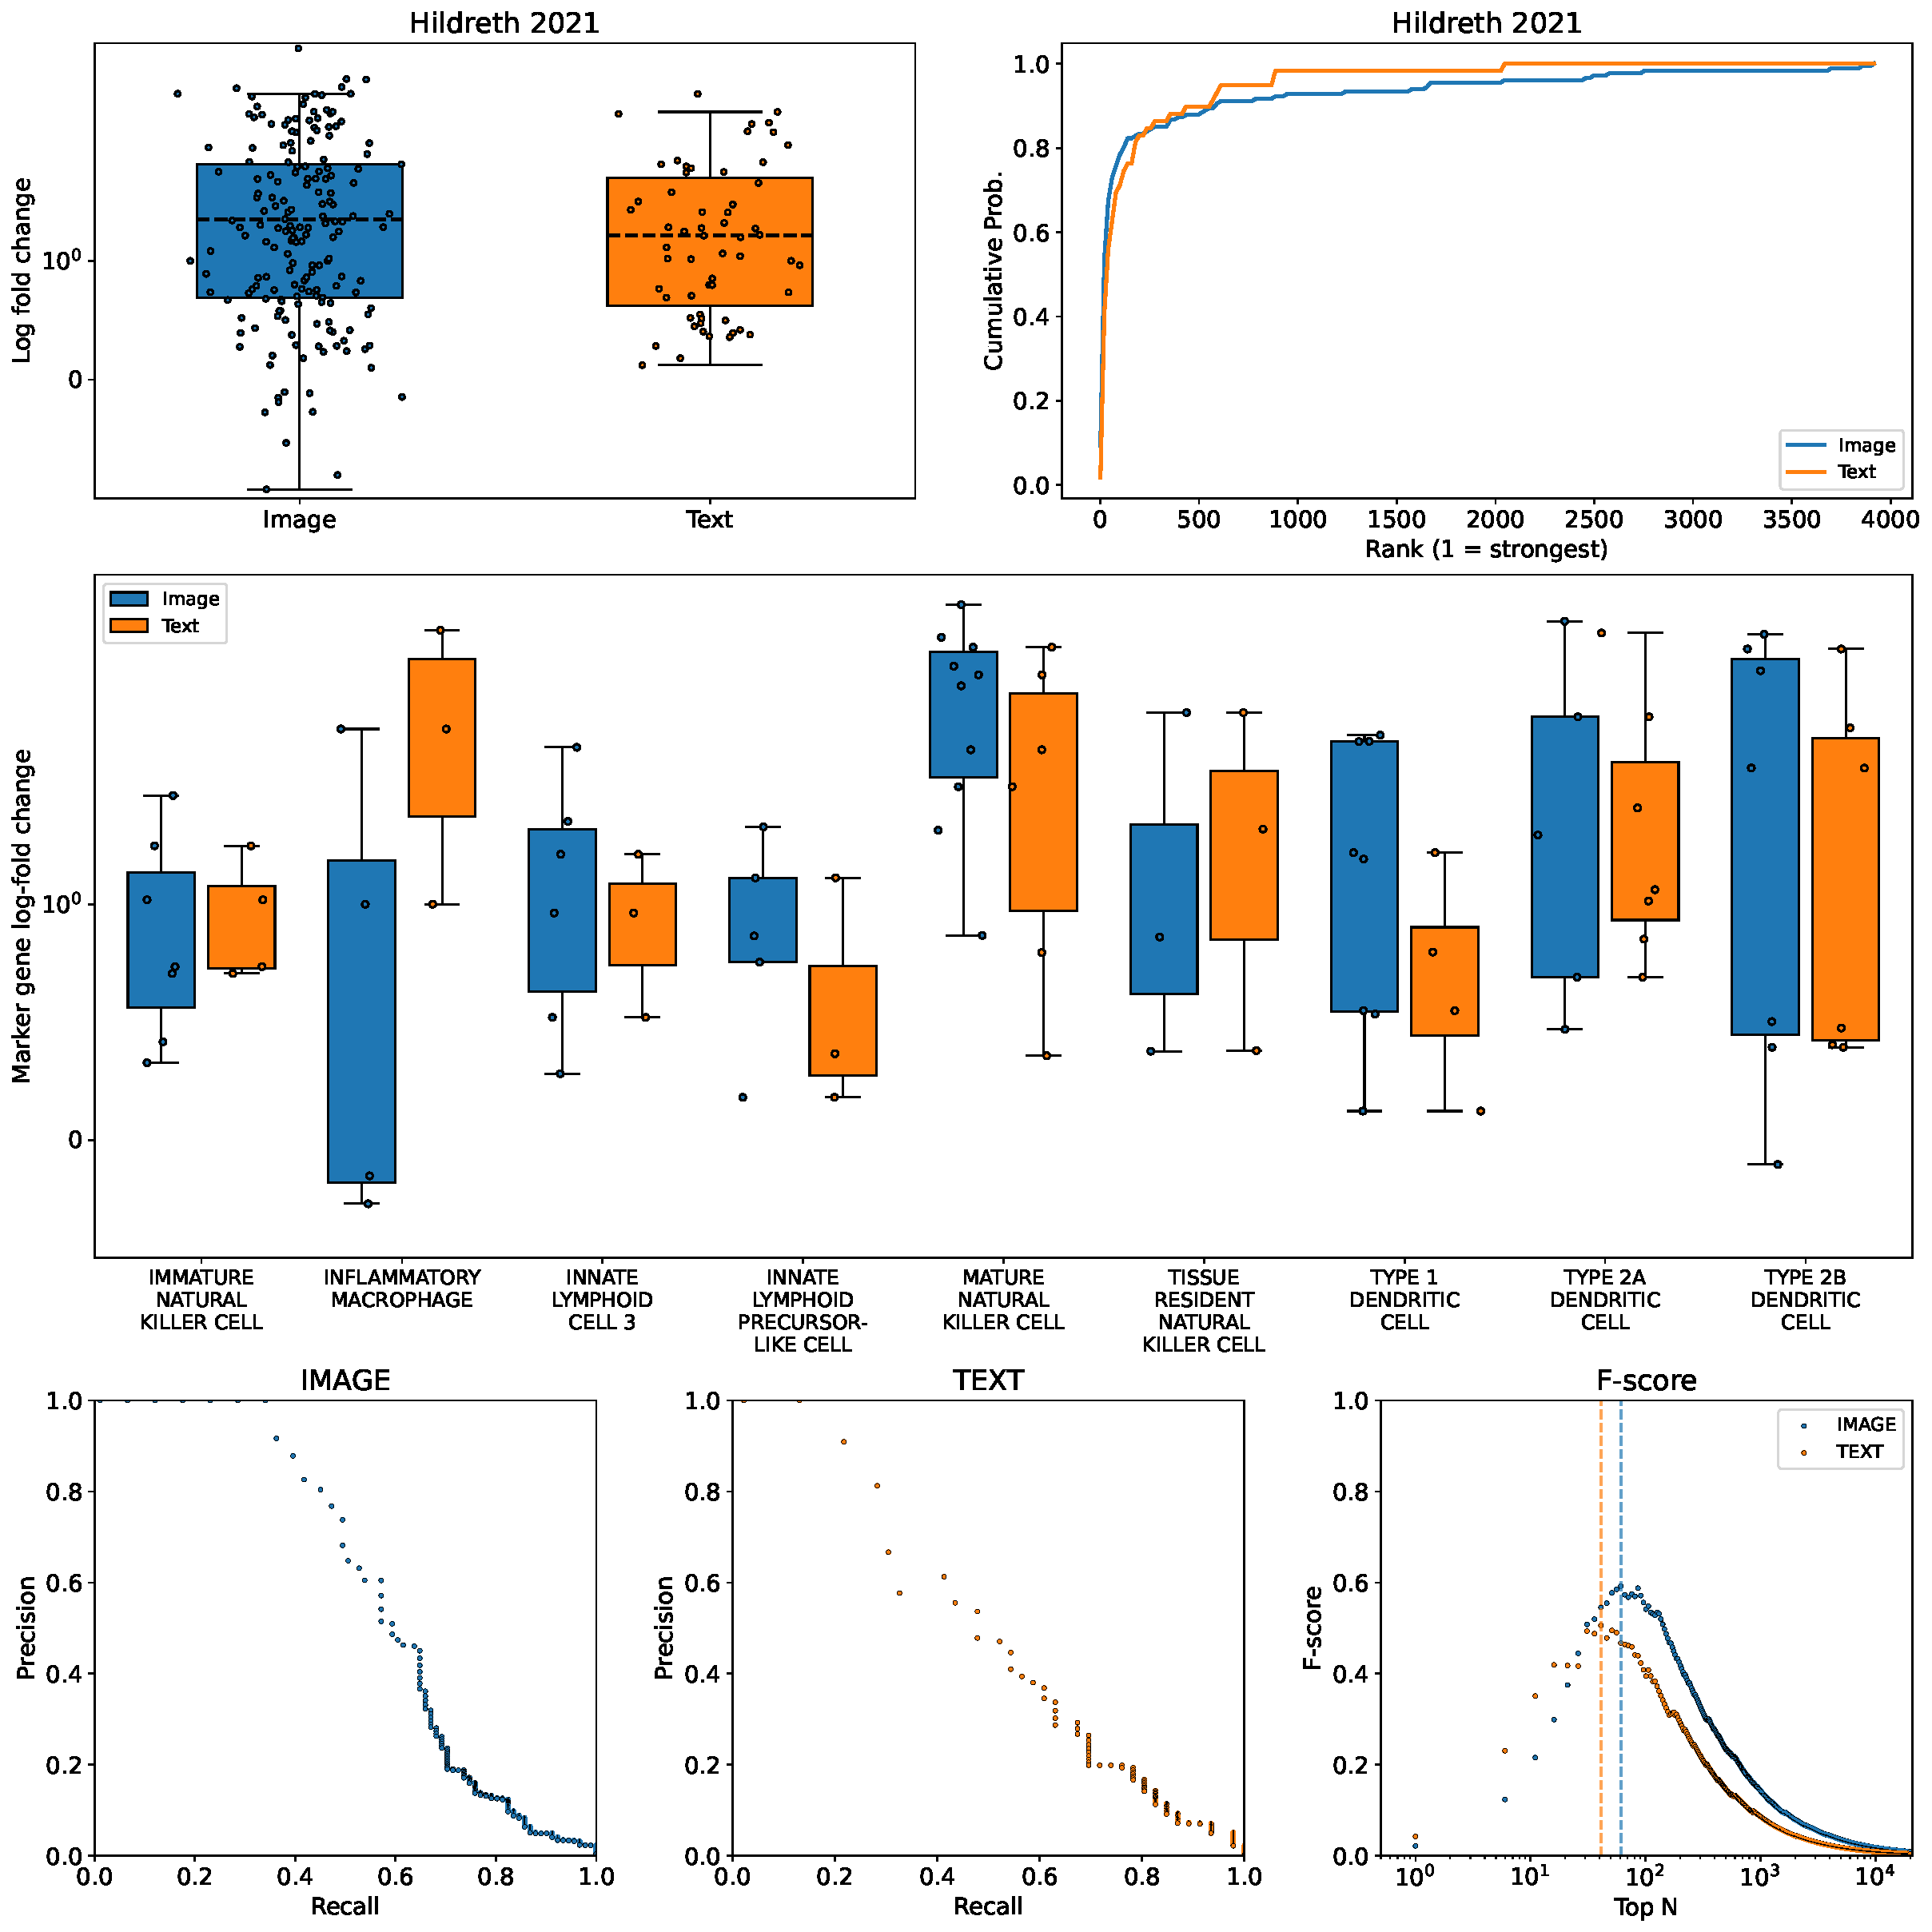
\includegraphics[width=\textwidth]{fig_hildreth_detail.pdf}
  \caption{\textbf{Marker gene selection strength for \citep{Hildreth2021}}. Top row shows log fold change distributions (left) and cumulative rank distributions (right) for discussed markers from images (blue) and text (orange). Middle row shows per-cell-type log-fold change distributions for image (blue) and text (orange) discussed markers. Bottom row shows precision--recall curves for image and text markers, and F-score as a function of the top-$N$ DEG threshold.}
  \label{fig:hildreth_detail}%
  \claim{fig-hildreth-detail}{}%
  \source{analysis/lfc_comparison.ipynb}%
\end{figure*}
 
\section{Results}

We first construct a benchmark dataset, called \texttt{LLMarkers} (for Large Language Model Markers), that connects each marker---extracted from the text and images of papers---to the specific DEG table from which it was derived. We then use \texttt{LLMarkers} to quantify the strength of markers that authors discuss in their papers, and compare the utility of LLM-based marker generation, selection, and extraction to expert-curated markers.

\begin{figure*}[ht!]
  \centering
  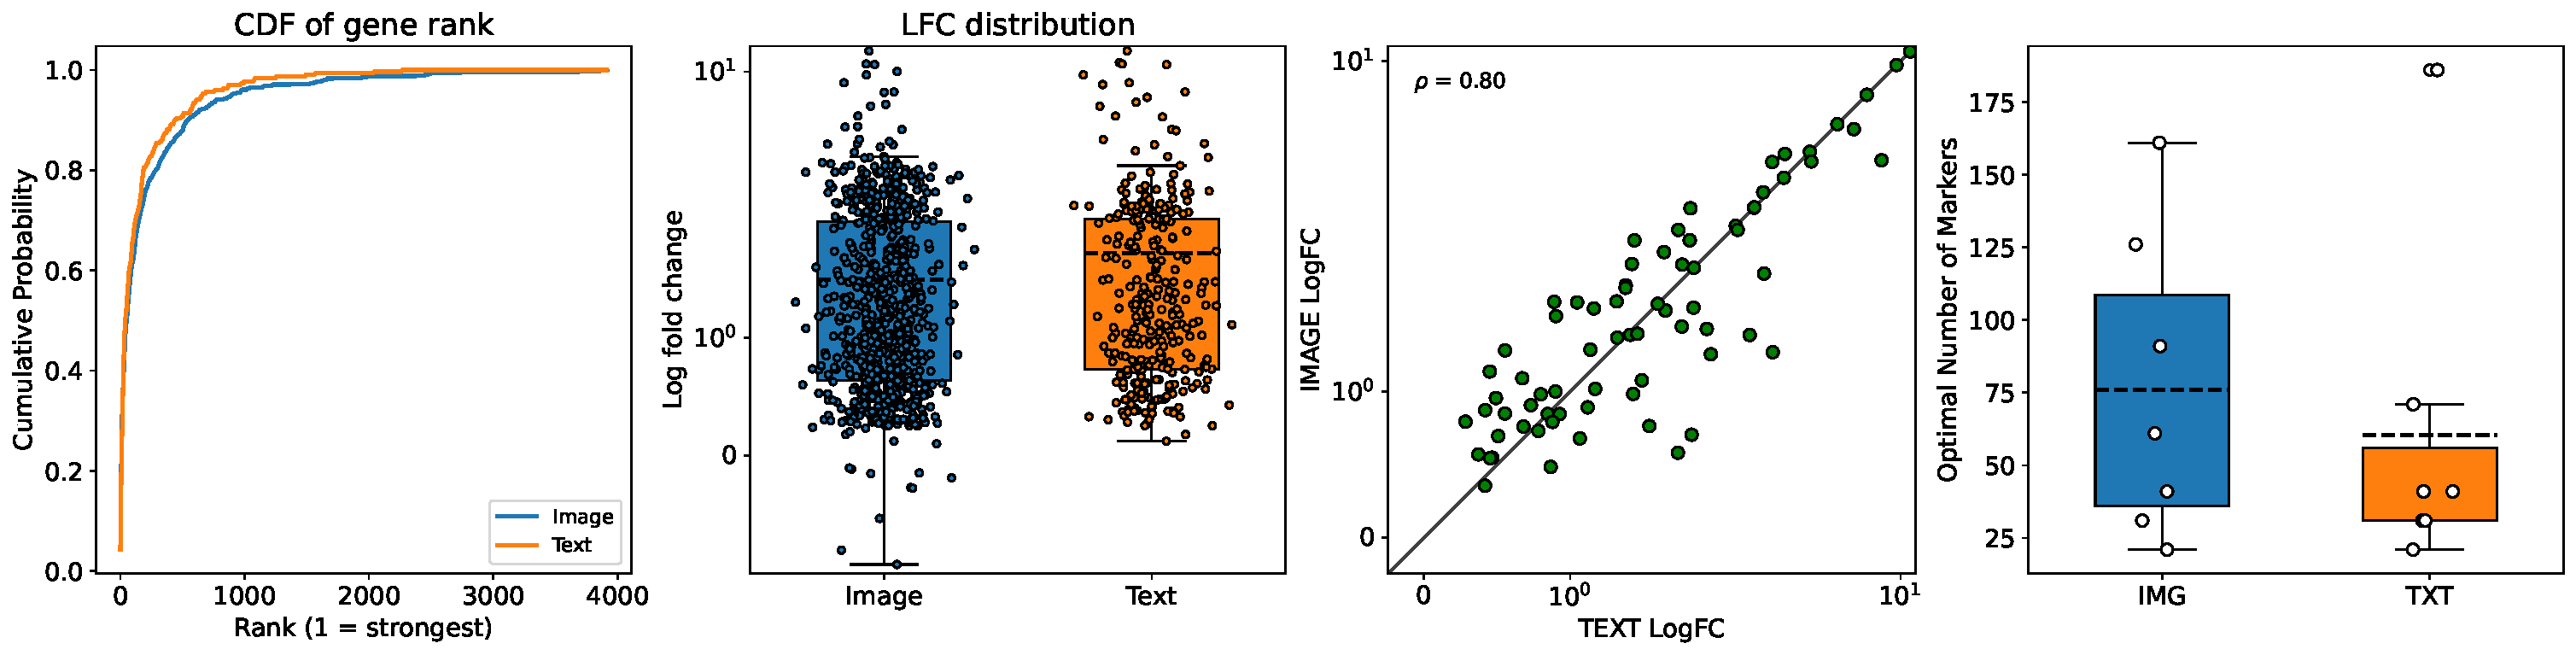
\includegraphics[width=\textwidth]{fig_marker_selection.pdf}
  \caption{\textbf{Marker gene selection across all seven datasets.} From left to right: cumulative distribution of DEG ranks for discussed markers from images and text; log fold change distributions for discussed markers; per-cell-type mean log-fold change of text-sourced versus image-sourced markers (each point is one cell type, diagonal is $y = x$); optimal number of markers (by F-score) for each dataset.}
  \label{fig:marker_selection}%
  \claim{fig-marker-selection}{}%
  \source{analysis/lfc_comparison.ipynb}%
\end{figure*}


\subsection{\texttt{LLMarkers} benchmark}
To evaluate the strength of markers that authors discuss in their papers, we assembled a dataset of marker genes from seven single-cell RNA-seq studies spanning six tissues: \texttt{adipose} (two studies) \citep{Emont2022,Hildreth2021}, \texttt{bone marrow} \citep{Zhong2020bone}, \texttt{retina} \citep{Gautam2021}, \texttt{lung} \citep{Adams2020}, \texttt{ovary} \citep{Wagner2020}, and \texttt{testis} \citep{Shamis2020}.

For each study, we extracted every cell type-marker gene association (Methods). For each marker, we annotated the position in the manuscript, or figure, from which the association was extracted. In addition, we annotated, for each marker, the specific data source from which the authors derived the marker, typically a DEG table containing the cell-type and gene name as well as the log-fold change of the expression of the gene. By pairing each marker with its respective DEG---taken from the study's supplementary tables---we created a relative expression strength-resolved list of marker genes (Table~\ref{tab:benchmark}). 

\claim{benchmark-summary}{\texttt{LLMarkers} contains 2{,}528 markers covering 168 cell types, 641 unique genes, and 1{,}560 unique cell type--gene pairs.}\source{analysis/benchmark_verification.ipynb} The fraction of markers drawn from text versus figures varies widely. Markers drawn from the text account for 69\% of records in \texttt{testis} and 60\% in \texttt{bone}, but only 6\% in \texttt{eye} and 8\% in \texttt{adipose (Emont)}. \claim{benchmark-modality}{Of the 1{,}560 unique pairs, 1{,}151 (74\%) appear only in figures, 256 (16\%) appear only in text, and 153 (10\%) appear in both. The number of marker genes per cell type ranges from 1 to 46, with a median of 6.}\source{analysis/benchmark_verification.ipynb}

\claim{benchmark-deg-totals}{The DEG tables contain 224{,}084 total entries across 39 supplementary data sources.}\source{analysis/benchmark_verification.ipynb} Not all human-curated markers appear in these tables. The marker overlap ranges from 18\% (\texttt{bone}) to 97\% (\texttt{lung}). In the \texttt{adipose (Emont)} dataset, for example, the authors describe PDGFRA as expressed across all six adipocyte stem and progenitor cell (ASPC) subpopulations, but the DEG table flags PDGFRA as differentially expressed for only one\footnote{The authors adopted ASPC (``adipose stem and progenitor cells'') as a unifying term for the Lin$^-$ stromal vascular fraction, noting that prior nomenclature---FAPs, ASCs, APCs, pre-adipocytes---is ``complicated and inconsistent'' \citep{Emont2022}. PDGFRA was identified as the common marker gene for this group, a choice driven by field consensus rather than differential expression ranking. Because PDGFRA is broadly expressed across all six subpopulations, it does not pass the DE threshold when comparing one subpopulation against the others, and appears in the DEG table for only ASPC~1. The second adipose dataset in our benchmark \citep{Hildreth2021} also reports PDGFRA as a marker for progenitor-like cells, but labels them ``adipocyte precursor cell'' and ``preadipocyte''---entirely different names for an overlapping biology. Of the 73 combined cell type names across both studies, only three are shared.}. More broadly, authors select markers not only from DEG rankings but also from prior knowledge, protein-level validation, or visual inspection of expression plots---criteria that formal differential expression tests may not capture. 

Because many studies include multiple supplementary DEG tables, the same cell type--gene pair can appear in more than one table with different fold changes. \claim{benchmark-sign-contradictions}{Of 544 human-curated marker pairs that appear in at least two DEG tables within the same study, 46 (8.5\%) show a sign contradiction where the gene is upregulated in one table and downregulated in another.}\source{analysis/benchmark_verification.ipynb} These contradictions are concentrated in datasets whose supplementary tables contain multiple cell-type comparisons (i.e. markers stratified by metadata like lean vs obese) 39\% of markers in \texttt{adipose (Hildreth)}, and 12\% in \texttt{lung}. By linking each marker to a specific DEG table, \texttt{LLMarkers} preserves these distinctions rather than collapsing them into a single binary (and potentially inconsistent) annotation.

\subsection{Expert marker curation}
When markers are reported, the data behind them---log fold changes (LFC), significance values, and the specific comparison that produced them---is often lost. We used \texttt{LLMarkers} to ask how the markers that authors choose to discuss relate to their underlying strength. We matched each human-curated marker to its entry in the corresponding DEG table, extracted the LFC, and then ranked the markers based on it.  \claim{expert-matched}{Across all seven datasets, 303 text and 763 image markers could be matched to DEG entries. All were statistically significant, but their fold changes varied (median LFC 1.19, IQR 0.66--2.00).}\source{analysis/gen_strength.ipynb}

In the \texttt{adipose (Hildreth)} dataset (Figure~\ref{fig:hildreth_detail}), discussed markers---from both images and text---had widely varying LFCs in aggregate (Figure~\ref{fig:hildreth_detail}, top row). The per-cell-type breakdown reveals that this variation arises from substantial cell type-specific variation. Some cell types (e.g.\ mature natural killer cells) had markedly higher LFCs than other cell types. And this trend was consistent between text and image markers (Figure~\ref{fig:hildreth_detail}, middle rows). 

Because extracted markers were highly ranked by their LFC, we asked whether a simple rank cutoff could substitute for expert curation. We computed precision--recall curves by treating the top $N$ DEGs as predicted markers and the human-curated set as truth, sweeping $N$ from 1 to 20{,}000. For the \texttt{Hildreth} dataset, the F-score (the harmonic mean of precision and recall) peaked at $N = 61$ for image markers and $N = 41$ for text markers (Figure~\ref{fig:hildreth_detail}, bottom row)---beyond this point, adding more DEGs diluted precision faster than it improved  recall. The markers discussed in \texttt{Hildreth} were strong, but strength alone did not fully explain their selection.

The same pattern held across all seven datasets (Figure~\ref{fig:marker_selection}). Discussed markers concentrated near the top of the DEG list but with large variance. \claim{expert-ranks}{The median rank was 40 for text and 50 for image, with about half falling within the top 50 DEGs (53\% text, 50\% image) and two-thirds within the top 100 (66\% text, 62\% image).}\source{analysis/lfc_comparison.ipynb} The remaining third of discussed markers came from deeper in the list, sometimes beyond rank 500. \claim{expert-spearman}{Although authors report different genes in their figures versus their text (median Jaccard 0.33), the per-cell-type LFCs are strongly correlated (Spearman $\rho = 0.80$, $p < 10^{-16}$, $n = 74$ cell types; Figure~\ref{fig:marker_selection}, middle right), suggesting that marker strength is a property of the cell type instead of the form in which they are reported.}\source{analysis/lfc_comparison.ipynb}

The precision--recall analysis across all seven datasets yielded similar results. \claim{expert-optimal-n}{The optimal $N$ averaged 76 for image markers and 60 for text markers, with peak F-scores of 0.51 and 0.44, respectively (Figure~\ref{fig:marker_selection}, last right).}\source{analysis/lfc_comparison.ipynb} In other words, a naive strategy of selecting the top 60--76 DEGs per cell type recovers at best half of the markers that domain experts chose to highlight---confirming that marker selection is not reducible to a rank threshold. Authors likely did not simply pick the most differentially expressed genes; marker selection reflects biological knowledge, prior literature, and protein-level validation.


\begin{figure*}[t]
  \centering
  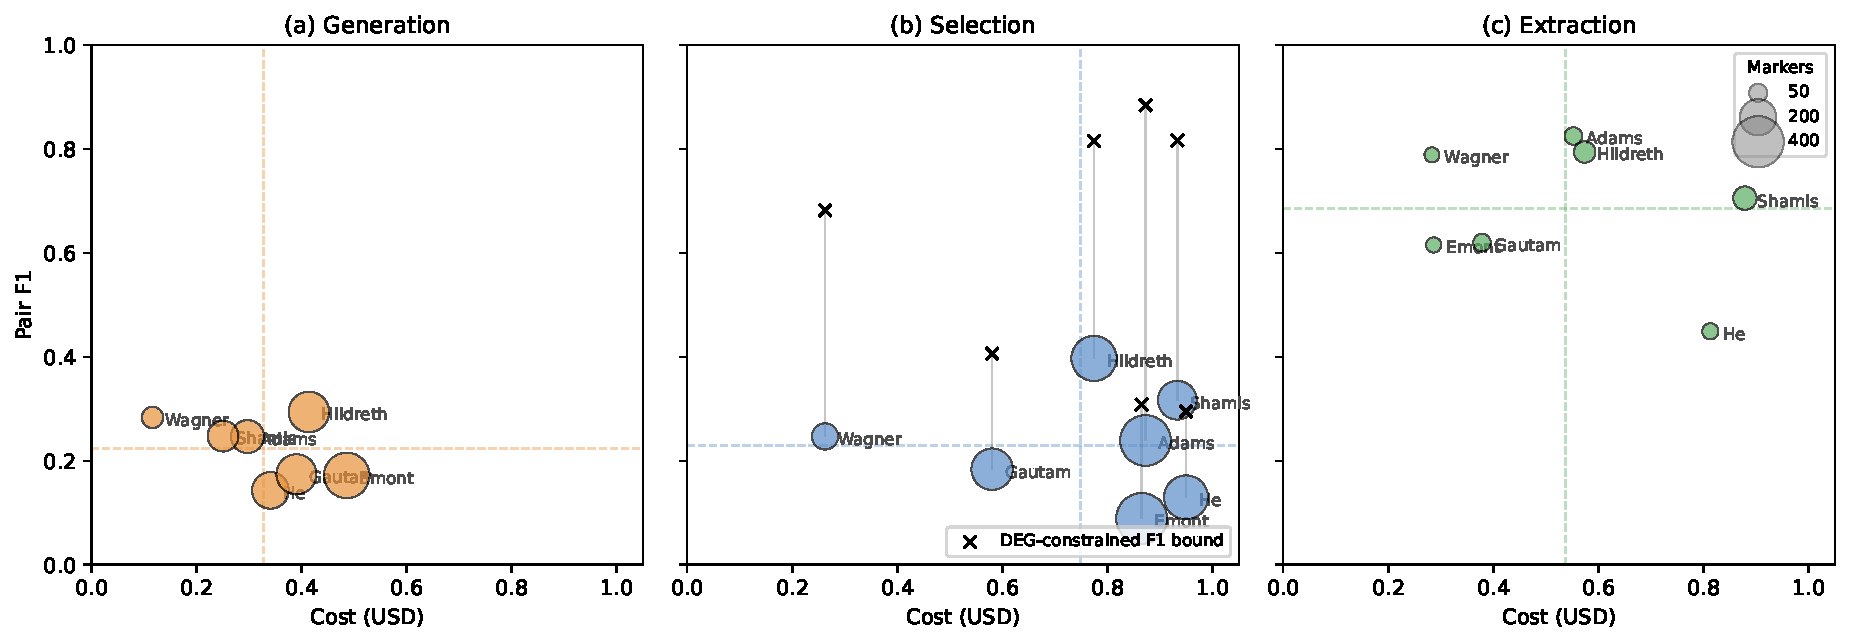
\includegraphics[width=\textwidth]{fig_llm_curation.pdf}
  \caption{\textbf{LLM curation tradeoff.} Cost versus fidelity for three LLM marker gene curation approaches across seven datasets, evaluated against text-sourced human annotations. Each point is one dataset; bubble size encodes the number of unique (cell type, gene) pairs produced. Dashed crosshairs mark the method mean on each axis. \textbf{(a)}~Generation from training knowledge. \textbf{(b)}~Selection from top-$N$ DEGs (at each dataset's optimal $N$). In panel (b), black \texttt{x} markers denote the max possible, DEG-constrained, F1 bound at that same $N$ (the maximum achievable F1 if the LLM could select only the recoverable human markers in the n-sized DEG). \textbf{(c)}~Extraction from manuscript text.}
  \label{fig:llm_curation}%
  \claim{fig-llm-curation}{}%
  \source{analysis/selection_analysis.ipynb}%
\end{figure*}


\subsection{LLM marker curation}

To assess whether LLMs have prior biological knowledge that informs consistent marker gene selection, we evaluated three LLM-based approaches to marker gene curation---generation, selection, and extraction---ordered by increasing dependence on study-specific data (Figure~\ref{fig:llm_curation}; Table~\ref{tab:llm_curation}). In generation, the model produces genes for named cell types relying only on training knowledge (or the reverse, where it produces a cell-type label for a given set of genes). In selection, the LLM receives the top $N$ DEGs per cell type and must select markers from that list. In extraction, the LLM reads the manuscript and identifies the marker--cell type associations made by the authors. (We evaluate text-only extraction here; image-based extraction is not tested.) To automate these tasks, we built \texttt{mrkr}, an open-source tool that prompts an LLM and verifies its output against source data.

% note we didn't include the tissue, maybe we shoud have?
We first asked whether an LLM could generate marker genes for cell types from training knowledge alone. Given a list of cell type names, \claim{gen-pairs}{the model generated 1{,}390 unique (cell type, gene) pairs across the seven datasets in \texttt{LLMarkers}. Most could be matched to markers in the corresponding DEGs, 845 (61\%) matched at least one entry, though non-uniquely since the LLM did not know which marker came from which table.}\source{analysis/ext_vs_gen.ipynb}\source{analysis/gen_strength.ipynb} Though many generated gene sets were genuine DEGs for the provided cell types, most were different from those that authors chose to highlight in their papers. Comparing LLM-generated cell type--marker gene pairs directly to expert-curated markers, \claim{gen-f1}{generation achieved a mean pair F1 of only 0.17 (Table~\ref{tab:llm_curation}a).}\source{analysis/ext_vs_gen.ipynb} The gap was largest in datasets where authors used study-specific cell type labels---numbered subtypes such as ``ADIPOCYTE 1'' through ``ADIPOCYTE 7'' in \texttt{adipose Emont} (pair F1~=~0.06) and ``LBM1'' through ``LBM3'' in \texttt{bone} (0.19)---whose markers depend on an association between experimental context and the label rather than canonical knowledge.

The differences between LLM-generated and expert-curated markers can partially be explained by the imprecise nature of cell-type labels. Cell type labels compress a molecular signature into a short name, which is practical, but lossy. So while LLMs struggled to identify specific genes for cell types labelled by author-specific nomenclature, the reverse test suggests that the model encodes genuine cell type--gene associations. Given anonymized gene lists---stripped of cell type names---\claim{gen-prediction}{the model predicted the correct label only 15\% of the time (27 of 181), but 72\% of predictions were semantically related (e.g., ``ROUND SPERMATID'' for ``ROUND SPERMATID CELL'').}\source{analysis/ext_vs_gen.ipynb} Even \texttt{bone} and \texttt{adipose Emont}---the two worst performers in the gene-list prediction task---achieved 67\% semantic accuracy in the reverse direction (18/27 and 30/45, respectively), compared with 4\% and 13\% exact match. A gene list is reasonably informative for the model to recognize a semantically similar cell type to those selected by experts, but the cell type name alone does not specify which genes an expert will choose. Normalizing cell type nomenclature across studies may help narrow the naming gap which may, in turn, improve evaluation of LLM-generated markers.

LLM-based marker gene generation relies entirely on training data, so we asked whether adding study-specific context could improve performance. We gave the model the top $N$ DEGs per cell type---with log fold changes and adjusted $p$-values---and asked it to select markers. We swept $N$ from 10 to 500. Across all runs, the LLM selected pairs that came from the DEG (mean 98\% of pairs were from the DEGs, Table~\ref{tab:llm_curation}). \claim{sel-f1}{At each dataset's optimal $N$, mean pair F1 was 0.16---comparable to generation's 0.17 (Table~\ref{tab:llm_curation}b; Figure~\ref{fig:llm_curation}b).}\source{analysis/selection_analysis.ipynb} \claim{sel-bound-eff}{Even relative to the DEG-constrained maximum F1 score, at the same dataset-specific $N$, selection reached only 20.2\% of the attainable max on average.}\source{analysis/selection_analysis.ipynb} \claim{sel-top200-cap}{On average, 66.7\% of text-sourced human-curated marker pairs are present within the top 200 DEGs, leaving one-third unrecoverable for any selection constrained to that list.}\source{analysis/selection_analysis.ipynb} As a control, we replaced cell type names with anonymous cluster labels and \claim{sel-anon}{the performance was unchanged (mean pair F1~=~0.16), confirming that cell type identity, alone, does not aid selection from ranked gene lists.}\source{analysis/selection_analysis.ipynb}

Generation and selection require the model to produce markers from its own knowledge. We asked whether LLMs could instead extract markers directly from the manuscript \citep{Booeshaghi_2026}. We built a tool, \texttt{mrkr}, that facilitates the use of LLMs for marker gene extraction. Using \texttt{mrkr}, \claim{ext-results}{we extracted 383 marker records (357 unique cell type--gene pairs) across seven datasets, far fewer than generation (1{,}390) or selection (1{,}901 at best $N$). Every extracted phrase matched the manuscript verbatim; 93\% of extraction records (357/383) had both cell type and gene label confirmed within the sentence}\source{analysis/llm_extraction_eval.ipynb} (mismatches arose when the model used a label not present verbatim in the sentence, e.g.\ labeling a cell type ``smooth muscle cells'' when the sentence uses the abbreviation ``SMCs'')). Because extraction operates on manuscript text only---not figures---we evaluated it against human curated text-based markers. \claim{ext-text-f1}{Mean pair F1 was 0.69, with precision of 0.71 and recall of 0.72. \texttt{Lung} (pair F1~=~0.82) and \texttt{ovary} (0.79) scored highest; \texttt{bone} scored lowest (0.45).}\source{analysis/llm_extraction_eval.ipynb} The low-scoring dataset likely reflects how the manuscript describes markers. Some authors tend to use dense parenthetical enumerations and gene-range shorthand (e.g.\ ``HOX9--11'') rather than explicit narrative statements to describe markers. The cell type label mismatches reflect inconsistent nomenclature which is contributed by the use of abbreviations, synonyms, and ad hoc naming conventions, making verifications fragile \citep{Booeshaghi_2026} \footnote{The nomenclature challenge likely contributed to the strong performance of LLM cell-type annotation in \citep{Xiao_2025} for broad cell types, which cleanly match standardized ontology terms, and underperformance for novel subtypes, which lose specificity in the ontology mapping process.}. When evaluated against all human annotations---including the 74\% of unique pairs appearing only in figures---\claim{ext-all-f1}{extraction pair F1 dropped to 0.34, because text-based extraction cannot recover markers described only in images.}\source{analysis/llm_extraction_eval.ipynb}


\begin{figure*}[ht!]
  \centering
  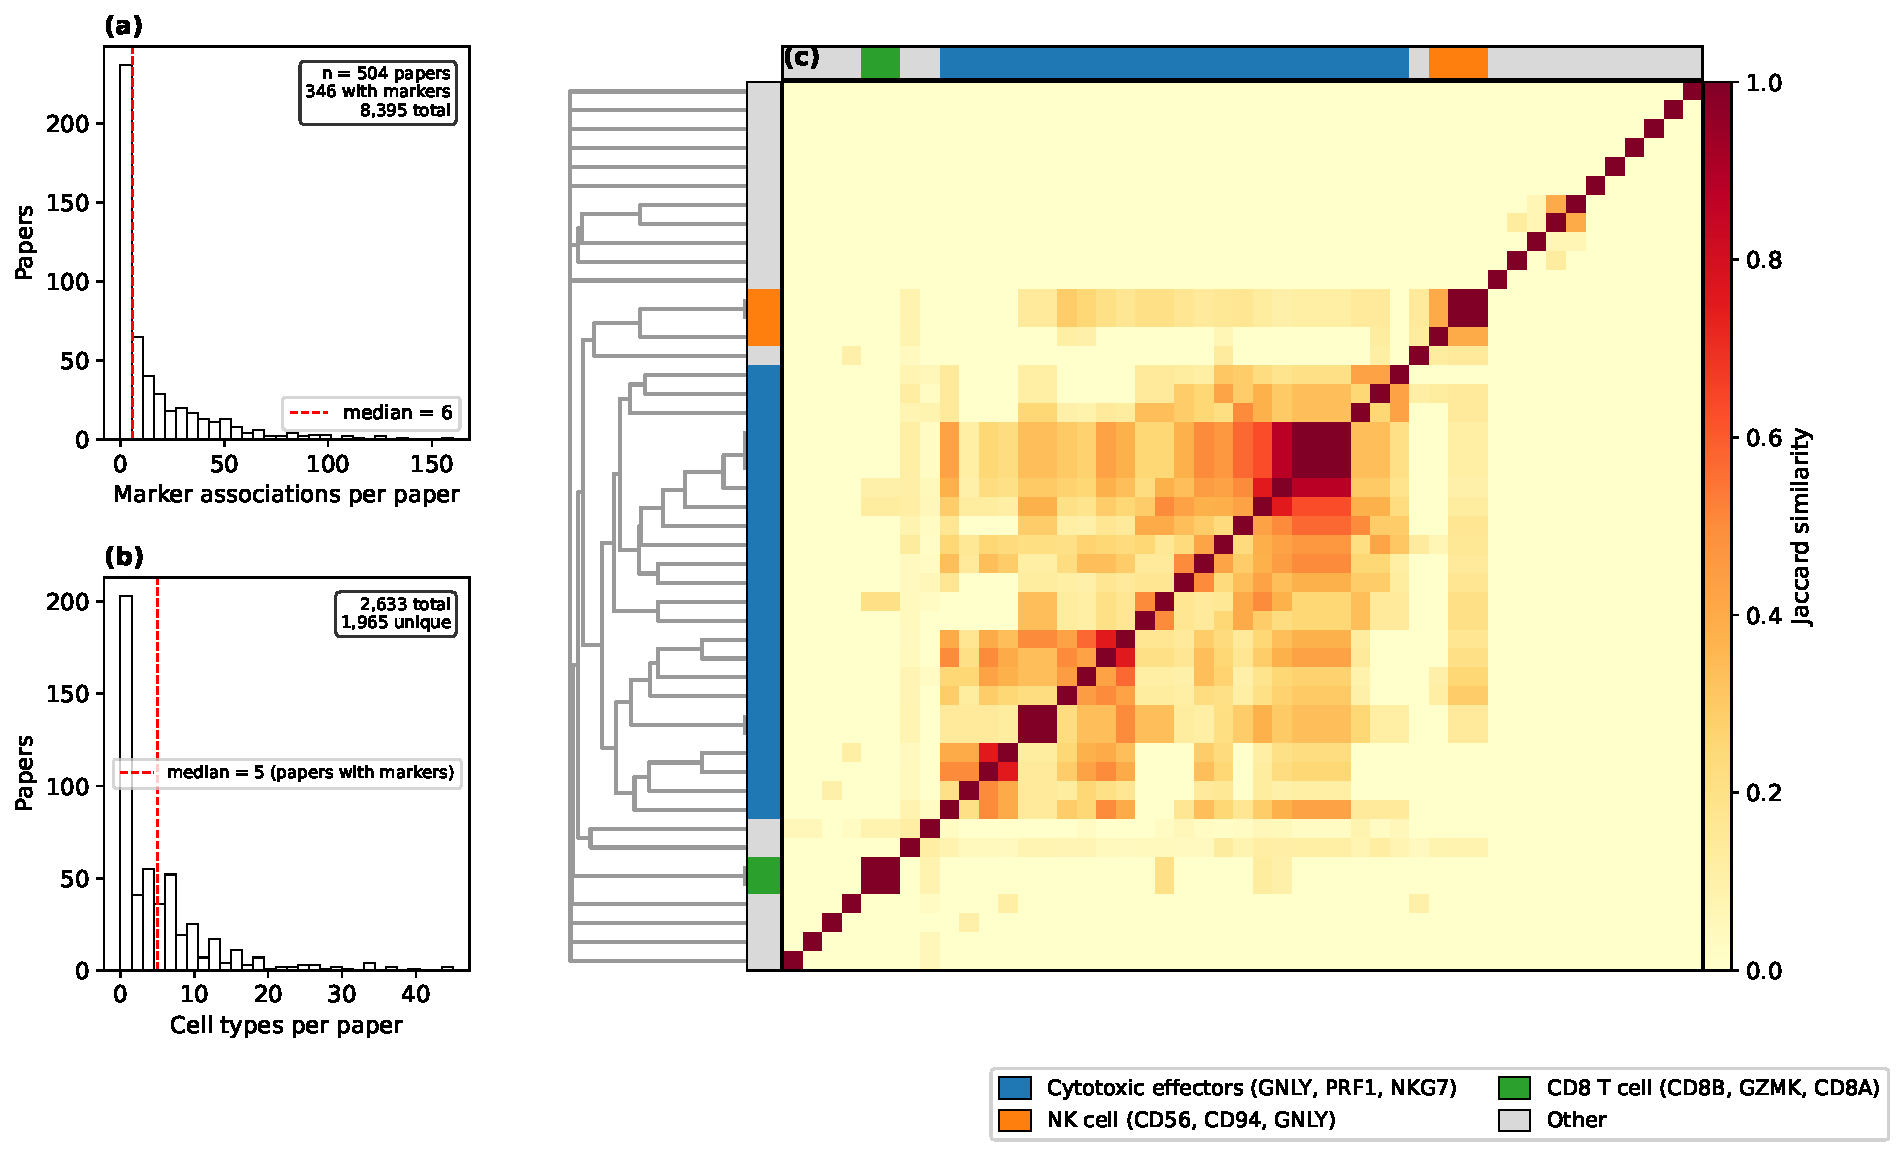
\includegraphics[width=0.9\textwidth]{biorxiv_immune_cluster.pdf}
  \caption{\textbf{bioRxiv cross-paper cell type similarity} \textbf{(a)}~Distribution of human marker associations per paper across 504 bioRxiv papers (median~=~8; 146 papers yielded no human markers). \textbf{(b)}~Distribution of mapped human cell types per paper (median~=~5 among papers with mapped markers; 1{,}965 unique cell type names total). \textbf{(c)}~Pairwise Jaccard similarity heatmap of the largest cluster (25 cell type names, 47 paper--celltype pairs), ordered by hierarchical clustering (average linkage). Color bars indicate sub-cluster identity after cutting at Jaccard distance 0.85. Block-diagonal structure reveals distinct immune sub-populations---cytotoxic effectors (GNLY, PRF1, NKG7), NK/NKT-associated cells (KLRD1, NCAM1, GNLY), and CD8 T~cells (CD8B, GZMK, CD8A)---that were merged by transitive linkage in the original connected component analysis but are separated by hierarchical clustering on the same marker gene vectors.}
  \label{fig:immune_cluster}%
  \claim{fig-immune-cluster}{}%
  \source{analysis/biorxiv_celltype_matching.ipynb}%
\end{figure*}

The three approaches to marker gene curation with LLMs show a tradeoff between fidelity and cost when all methods are evaluated against text-sourced human annotations (Figure~\ref{fig:llm_curation}). \claim{method-costs}{Marker gene generation is cheapest (\$2.30 total, \$0.33 per paper) but recovers only canonical markers that overlap modestly with any particular study (the reverse direction---predicting cell type labels from gene lists---is more accurate). Selection costs the most (\$5.94, \$0.85 per paper) yet performs no better, showing that DEG rankings alone cannot substitute for expert reasoning and knowledge. Extraction falls between the two in cost (\$3.77, \$0.54 per paper) while achieving the highest fidelity}\source{analysis/selection_analysis.ipynb}, because it recovers the specific associations that authors chose to highlight---including context-dependent markers that neither generation nor selection has access to. For capturing what a paper claims, extraction is the appropriate approach; generation complements it by surfacing canonical markers that may not appear in any particular manuscript.


\subsection{Automated extraction from bioRxiv}

LLMs effectively extracted marker genes and LLM-generated cell-type labels showed that marker genes carry enough signal to identify cell types independent of their names. We therefore asked whether extraction could scale to a large corpus and whether the resulting marker genes could be used to resolve ambiguous cell-type labels across papers. We ran \texttt{mrkr extract} on 504 bioRxiv preprints retrieved from bioRxiv (see Methods for selection criteria). Each paper was converted from JATS~XML to markdown and processed with text-only extraction.
All extracted records are available through an interactive browser at \url{https://sbooeshaghi.github.io/llmarkers/}.

\claim{biorxiv-totals}{Of the 504 papers, 421 (84\%) yielded at least one marker gene--cell type association; the LLM did not identify marker gene claims in the remaining 83 papers. Across the 421 papers, \texttt{mrkr} extracted 12{,}501 marker gene--cell type associations covering 3{,}906 unique genes, 2{,}720 unique cell type names, and 11{,}231 unique (cell type, gene) pairs.}\source{analysis/biorxiv_summary.ipynb} Human markers were most prevalent (71\%), followed by mouse (19\%), with 18 additional species appearing at lower frequency. \claim{biorxiv-verification}{All 12{,}501 extractions were verified as verbatim substrings of their manuscripts. Of these, 89\% of cell-type marker gene pairs were fully verified, meaning that the cell type label and gene label were both confirmed within the extracted text (Methods). The 11\% partial failures were almost entirely cell-type label mismatches (10\%), where the cell type could not be aligned within the extracted sentence, typically because the model normalized the name differently than how it appeared in the manuscript.}\source{analysis/biorxiv_summary.ipynb}

\claim{biorxiv-cost}{The total cost was \$92 for all 504 papers (\$0.18 per paper on average), consuming 6.6M input tokens and 2.4M output tokens. The summed per-paper processing time was 367.6 minutes (43.9 seconds per paper on average).}\source{analysis/biorxiv_summary.ipynb}

To enable consistent cross-paper comparison, we mapped extracted gene symbols to Ensembl identifiers using a reference built from Ensembl GRCh38.114 (Methods) and restricted our analyses to mapped human markers only. \claim{biorxiv-mapping}{Of the 8{,}921 human markers across 358 papers, 8{,}395 (94\%) mapped to Ensembl identifiers. Restricting to mapped entries yielded 2{,}566 unique Ensembl IDs across 1{,}965 unique cell type names from 346 papers.}\source{analysis/biorxiv_celltype_matching.ipynb} The unmapped entries included protein names (CD3, KI67) and Unicode variants of Greek-letter gene names (IFN$\gamma$, IL1$\beta$).

The 8{,}395 mapped human markers use 1{,}965 distinct cell type names for what is likely a far smaller number of biological cell types, many of which may be related or identical across studies. To quantify this nomenclature heterogeneity, we computed pairwise Jaccard similarity between the marker gene sets of all mapped human cell types across papers. \claim{biorxiv-clusters}{Among cross-paper cell-type pairs with different names, 182 pairs exceeded a Jaccard threshold of 0.5, and 651 exceeded 0.3. These include abbreviation variants (``SMC'' and ``smooth muscle cell'' sharing ACTA2, CNN1, MYH11, TAGLN), plural forms (``B~cell'' and ``B~cells''), and biologically equivalent labels (``mesenchymal stem cell,'' ``MSCs,'' and ``IMSCs'' all referring to the same lineage). At a Jaccard threshold of 0.4, connected component analysis grouped these into 43 clusters, 22 of which contained three or more distinct names.}\source{analysis/biorxiv_celltype_matching.ipynb}

As expected from the Jaccard-based grouping, within-cluster similarity far exceeded between-cluster similarity \claim{biorxiv-cluster-quality}{(mean pairwise Jaccard 0.35 vs.\ 0.004).}\source{analysis/biorxiv_celltype_matching.ipynb} Silhouette analysis---an independent measure of cluster quality---revealed a size--quality tradeoff: small clusters of 2--5 cell types achieved silhouette scores of 0.4--0.6, while the largest cluster scored near zero, indicating that transitive linkage had merged distinct cell types.

Hierarchical clustering within the largest cluster recovered an immune cell hierarchy (Figure~\ref{fig:immune_cluster}). At a Jaccard distance threshold of 0.85, the 47 paper--celltype pairs separated into 20 sub-clusters. The three largest biologically interpretable sub-clusters correspond to cytotoxic effectors (GNLY, PRF1, NKG7; 24 pairs), NK/NKT-associated cells (KLRD1/CD94, NCAM1/CD56, GNLY; 3 pairs), and CD8 T~cells (CD8B, GZMK, CD8A; 2 pairs) (Supplementary Table~\ref{tab:immune_subclusters}). Per-pair silhouette scores show that the separation is imperfect. NK/NKT-associated cells contain cytotoxic effector genes (GNLY, GZMB, PRF1) alongside canonical NK markers (CD94, CD56) and had near zero silhouette scores indicating that they sit on the boundary between the cytotoxic effector and NK/CD8 sub-clusters.

That standard hierarchical clustering on text-extracted markers, alone, recovers this known biology indicates that LLM extraction captures genuine molecular signatures from unstructured text. Despite sharing enough markers to cluster together, these sub-populations carry distinct labels across papers. The same principle observed in the benchmark---where marker genes identified the semantically similar cell type label 72\% of the time despite a 15\% exact name match---operates here at corpus scale. Marker genes reveal biological relationships that string matching on names alone would miss. This suggests an approach to overcome the nomenclature problem that motivated this analysis.

At the same time, cross-paper concordance for even well-defined cell types was modest. \claim{biorxiv-monocyte}{Monocytes appeared in 29 papers but shared a mean Jaccard of only 0.063.}\source{analysis/biorxiv_celltype_matching.ipynb} This low concordance is likely caused by diversity in study context, including rheumatoid arthritis, Sjogren's disease, HIV vaccine response, AML, interferon signaling, COVID-19, and other settings (Supplementary Table~\ref{tab:monocyte_papers}). Each paper likely reports monocyte markers relevant to its experimental question instead of a basal monocyte profile. 

Text-extracted markers therefore serve as a linked index across the literature where cell-types can be aligned across papers by finding matching marker genes, independent of the nomenclature used to name the cell type. But complete marker gene profiles require the underlying data---differential expression tables, expression matrices---tied to the experimental context from which they were derived.

\subsection{Finding cell type marker genes}


\balance
\section{Discussion}

Scientists describe cell types with binary, qualitative marker genes. While practical for compressing large amounts of quantitative measurements into a binary signal, this compression is lossy. A binary marker carries a minimal record of how strong the gene was, which comparison produced it, or which experimental context gave it meaning. The \texttt{LLMarkers} benchmark reveals that these binary markers cannot be fully recovered by a simple statistical test and cutoff from a DEG table. A rank threshold on differential expression recovers at best half of the markers that authors highlight from a particular study. The rest come from deeper in the DEG list, from prior knowledge, or from outside the table entirely. Marker selection requires biological judgment that cannot be reconstructed from statistics alone---a finding confirmed by our LLM experiments, where giving the model the full DEG ranking with fold changes and $p$-values (selection) performed no better than giving it cell type names alone (generation).

Human experts have demonstrated that they have internalized real cell type--gene associations, and so have LLMs. The experiment where the model identified semantically related cell types from anonymized gene lists 72\% of the time confirms this. But this knowledge is drawn from a consensus across the literature rather than grounded in a specific experiment. When asked to generate markers for named cell types, the model produced biologically plausible genes that overlap with, but do not replicate, any particular study's discussed genes. The LLM has a specificity problem in that it cannot know which genes an author chose to highlight without knowing about the experimental context---in other words, without reading the paper.

Extraction addresses this problem by recovering the marker genes directly from the manuscript---the sentences in which authors state that a gene marks a cell type. Each extraction is verifiable against the text and traceable to a specific sentence. When paired with the DEG table, as in the \texttt{LLMarkers} database, the marker can be further quantified. But extraction is not perfect. Text verification is challenging when authors use abbreviations, ad hoc nomenclature, and dense parenthetical styles that can obscure the exact name of a cell type or gene.

The challenge of connecting markers to their context is compounded by highly variable cell type nomenclature. Often the same biological cell type appears under different names across papers, while the same-named cell type can have different markers derived from different experimental contexts. In our analysis, monocytes appeared in 29 papers and had a mean pairwise Jaccard of 0.063, because each paper reported whichever monocyte markers were relevant to its experimental question. A binary catalogue that treats these situations as the same may obscure important biological findings.

Despite these naming issues, binary markers can help bridge the nomenclature gap. Hierarchical clustering on text-extracted markers, without any name standardization, recovered a known immune cell hierarchy from 1,965 distinct cell type names across 346 papers. This demonstrates that even coarse, context-dependent markers are informative enough for identifying which papers studied related cell types despite using different names. In this way, LLM-based marker gene extraction can provide a linked index into the literature (which papers discuss which cell types, supported by which evidence) and a bridge across inconsistent nomenclature.

These findings suggest a path toward marker gene resources that preserve what binary labels discard. Each marker entry could point to the data that generated it, the sentence in the study that described it, and the experimental context relevant to its generation. By offering machine-readable metadata for marker genes, such records could serve as structured training data for models that reason about cell type identity in context---for example, predicting which markers are likely to replicate in a new tissue or condition based on results from prior studies.

Ultimately, this study argues that the link between a marker gene and its underlying evidence is worth preserving. Binary markers are useful shorthand, but they discard the experimental context that determines which genes are relevant and why. LLM-based extraction offers a practical path to establishing this link at scale both retroactively and proactively. As the volume of single-cell data grows, we envision marker gene resources that move beyond flat lists of cell type--gene pairs toward machine-readable records that preserve provenance, quantitative strength, and experimental context---enabling researchers to query not just what markers exist, but where they came from, how strong they are, and in what setting they were generated.

% fold this in to the discussion
\section{Limitations}
Several limitations constrain the current work. Our extraction pipeline operates on manuscript text only; because 74\% of unique marker pairs in the benchmark appear exclusively in figures, text-only extraction misses the majority of visually communicated markers and markers identifiable only by re-analyzing the underlying data. Verification relies on exact substring matching and subword alignment, so abbreviations and ad hoc naming conventions produce false negatives even when extractions are semantically correct. The benchmark comprises seven studies curated by a single annotator, gene mapping covers only human genes (Ensembl GRCh38.114), and all experiments used a single LLM (Claude Opus). Extending extraction to figures and the raw data, expanding the benchmark, and testing across models are natural next steps.

\clearpage
\newpage
\onecolumn
\appendix

\section{Supplementary Material}

% \begin{figure*}[ht!]
%   \centering
%   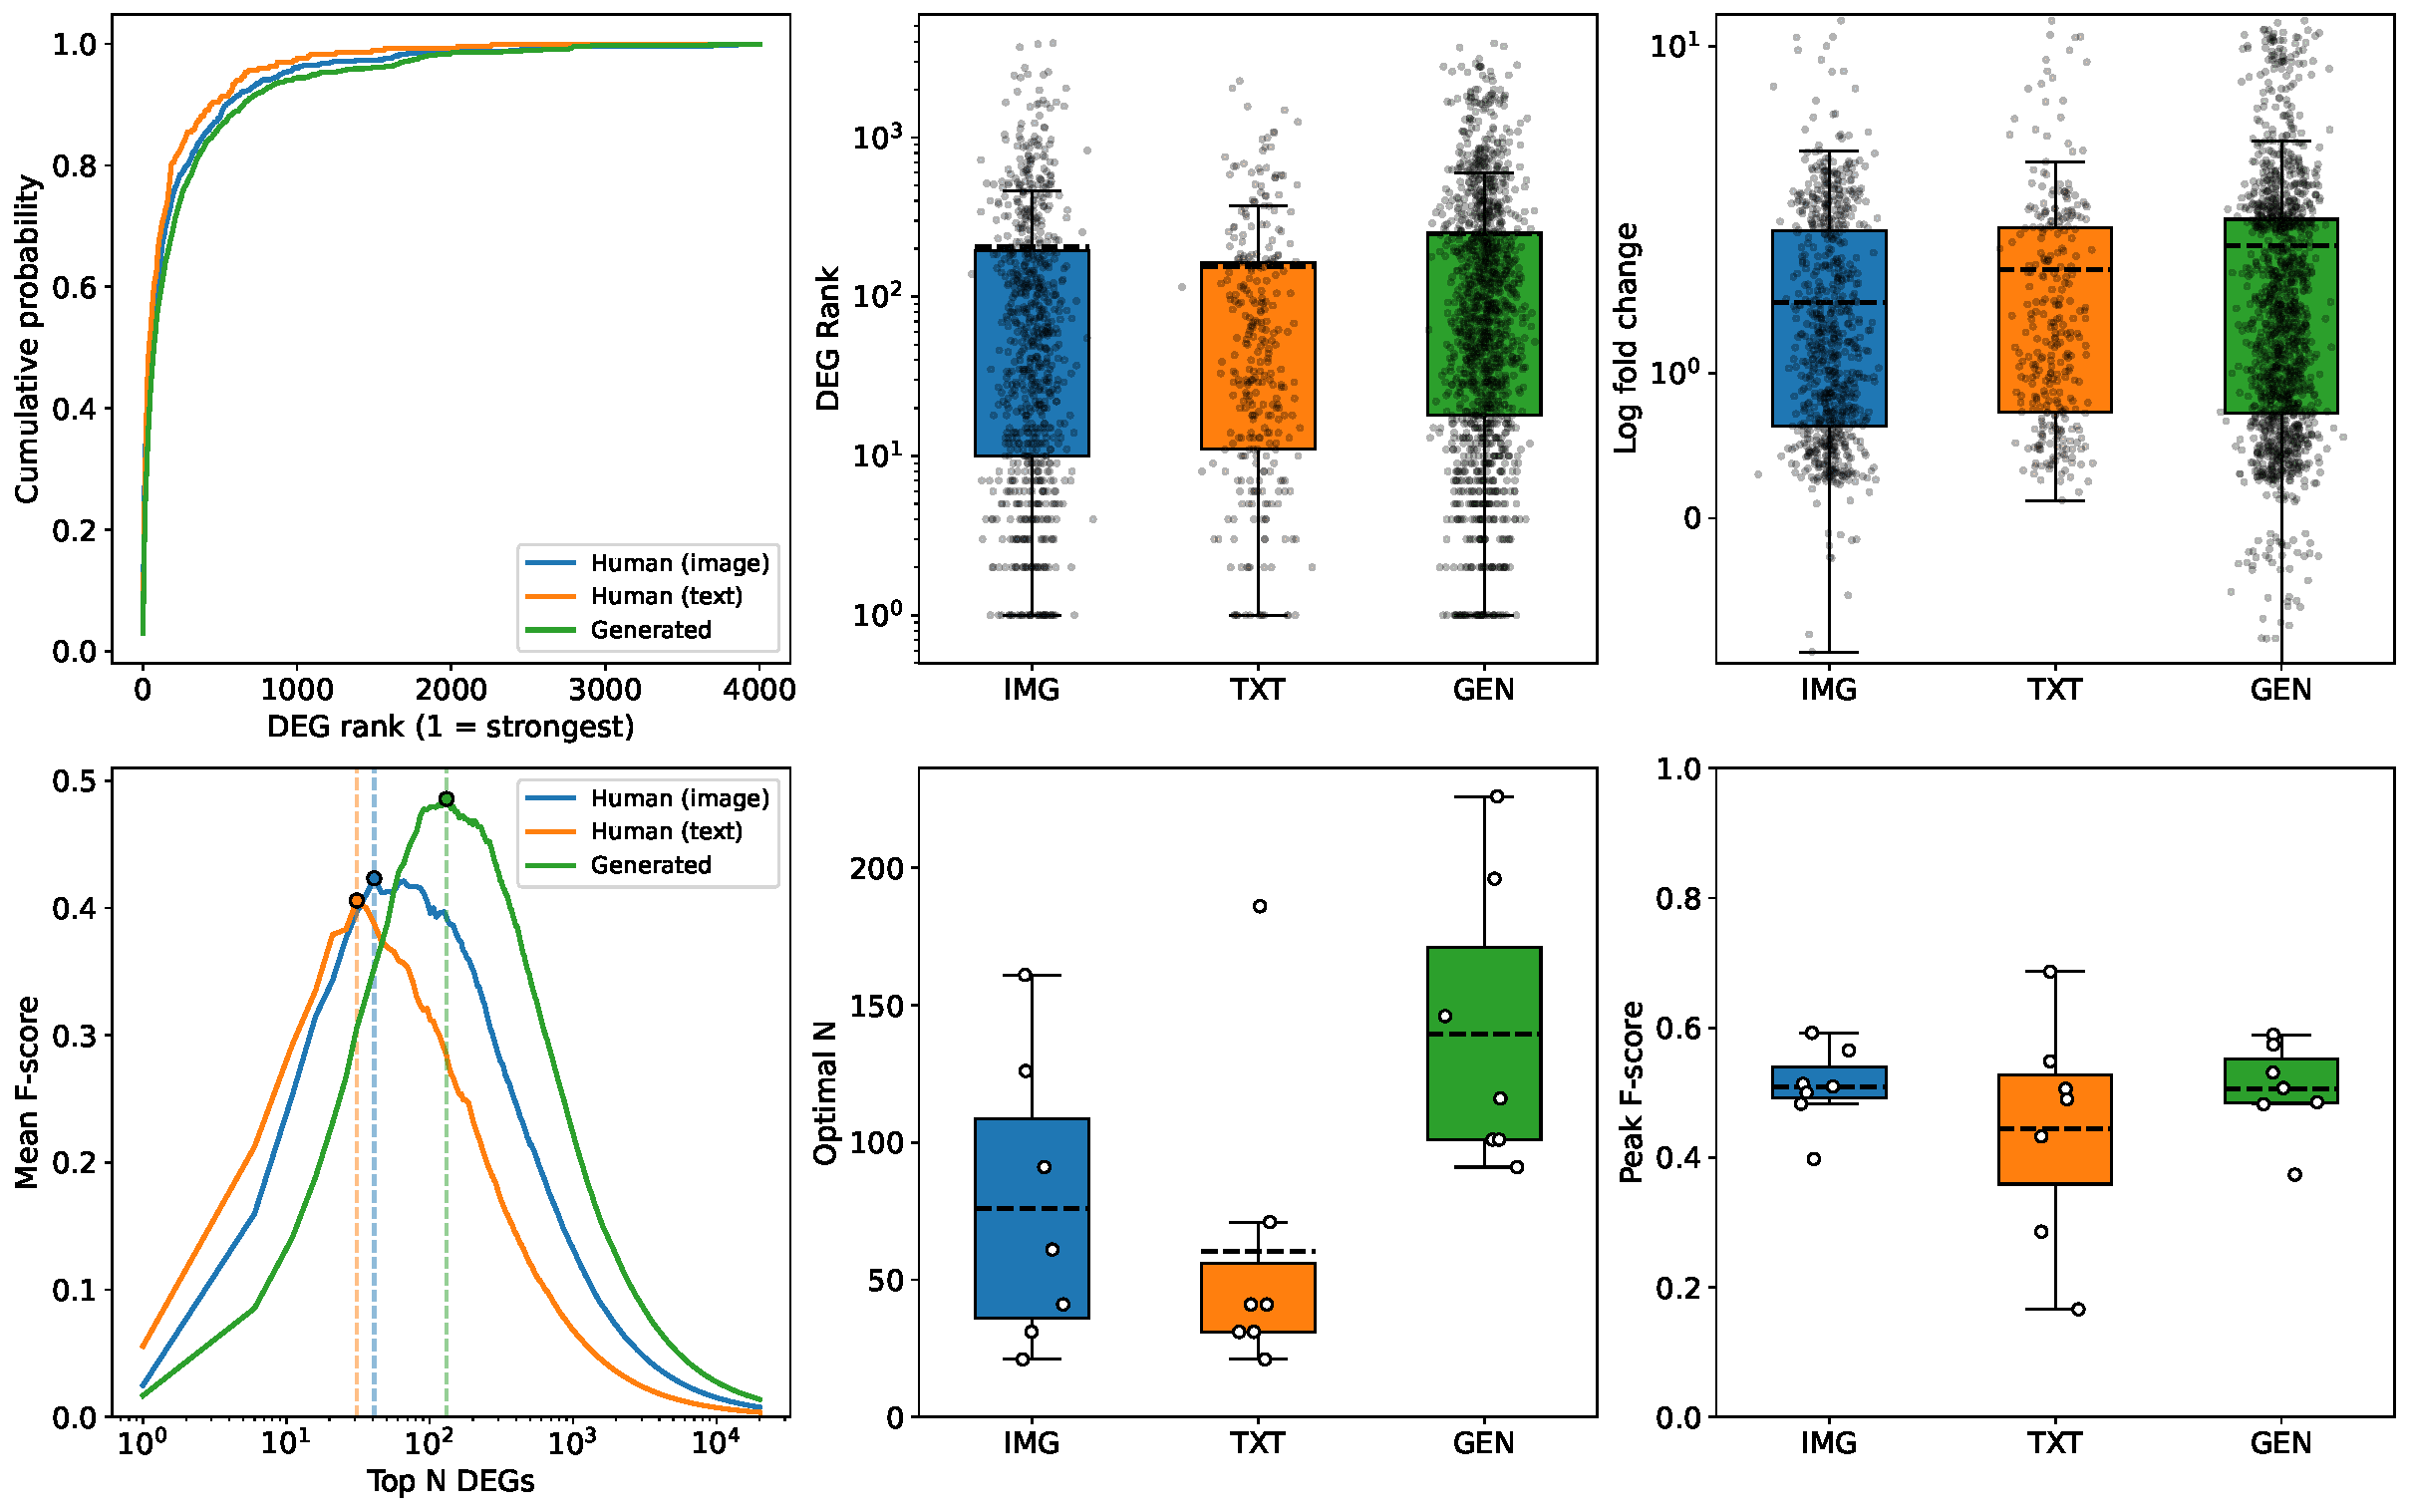
\includegraphics[width=\textwidth]{fig_gen_comparison.pdf}
%   \caption{Comparison of LLM-generated markers with expert-curated markers across all seven datasets. \textbf{(a)}~Cumulative distribution of DEG ranks for image-sourced (blue), text-sourced (orange), and generated (green) markers. \textbf{(b)}~Log fold change distributions by marker source. \textbf{(c)}~Per-cell-type mean LFC for generated versus human-curated markers. \textbf{(d)}~Precision--recall curves for the top-$N$ DEG threshold, treating generated markers as truth. \textbf{(e)}~F-score as a function of top-$N$ threshold. \textbf{(f)}~Optimal $N$ per dataset for image, text, and generated marker sets.}
%   \label{fig:gen_comparison}%
%   \claim{fig-gen-comparison}{}%
%   \source{analysis/gen_strength.ipynb}%
% \end{figure*}

\begin{table*}[ht!]
  \centering
  \caption{\textbf{LLM marker gene curation}. All runs used Claude (claude-opus-4-6). P, R, and F1 are precision, recall, and F1 on (group\_name, feature\_id) pairs evaluated against text-sourced human annotations. \textbf{$N$}: number of unique pairs produced. \%DEG: percentage of produced pairs found in the matching DEG table (by data\_id). Rank: median DEG rank of matched pairs. Opt~$N$: DEG rank threshold maximizing F-score. DEG columns require a data\_id link and are not available for generation (---). Cost: total API cost in USD. Time: wall-clock minutes. Bottom row shows means across datasets. \textbf{(a)}~Generation. The model was given cell type names only. Pred.\ Acc.: fraction of cell types correctly identified from anonymized gene lists. \textbf{(b)}~Selection. The model was given the top DEGs per cell type. Best~$N$: number of top DEGs maximizing pair F1 per dataset. \textbf{(c)}~Extraction. The model was given the manuscript text. Verified: fraction of extractions where source rationale, group label, and feature label were all confirmed.}
  \label{tab:llm_curation}%
  \claim{tab-llm-curation}{}%
  \source{analysis/ext_vs_gen.ipynb}%
  \source{analysis/selection_analysis.ipynb}%
  \source{analysis/llm_extraction_eval.ipynb}%
  \small
  \setlength{\tabcolsep}{4pt}

  \textbf{(a) Generation}
  \vspace{2pt}
  
  \begin{tabular}{@{}l c r ccc ccc r r@{}}
  \toprule
  Dataset & Pred. \% & $N$ & \%DEG & Rank & Opt $N$ & P & R & F1 & Cost (\$) & Time (min) \\
  \midrule
  \texttt{Adipose (Emont)}    & 13 & 317 & -- & -- & -- & 0.03 & 0.37 & 0.06 & 0.48 & 3.2 \\
  \texttt{Adipose (Hildreth)} & 10 & 249 & -- & -- & -- & 0.13 & 0.48 & 0.20 & 0.41 & 2.8 \\
  \texttt{Bone (He)}          & 4  & 203 & -- & -- & -- & 0.14 & 0.30 & 0.19 & 0.34 & 2.3 \\
  \texttt{Eye (Gautam)}       & 13 & 243 & -- & -- & -- & 0.04 & 0.42 & 0.07 & 0.39 & 2.6 \\
  \texttt{Lung (Adams)}       & 40 & 165 & -- & -- & -- & 0.07 & 0.33 & 0.11 & 0.29 & 2.0 \\
  \texttt{Ovary (Wagner)}     & 29 &  69 & -- & -- & -- & 0.26 & 0.49 & 0.34 & 0.11 & 0.8 \\
  \texttt{Testis (Shamis)}    & 16 & 144 & -- & -- & -- & 0.20 & 0.24 & 0.22 & 0.25 & 1.7 \\
  \midrule
  Mean               & 15 & 199 & -- & -- & -- & 0.13 & 0.37 & 0.17 & 0.33 & 2.2 \\
  \bottomrule
  \end{tabular}
  
  
  \vspace{8pt}
  \textbf{(b) Selection}
  \vspace{2pt}
  
  \begin{tabular}{@{}l r r rrr ccc r r@{}}
  \toprule
  Dataset & Best $N$ & $N$ & \%DEG & Rank & Opt $N$ & P & R & F1 & Cost (\$) & Time (min) \\
  \midrule
  \texttt{Adipose (Emont)}    & 200 & 371 &  97 & 17 & 11 & 0.03 & 0.33 & 0.05 & 1.53 &  4.4 \\
  \texttt{Adipose (Hildreth)} & 400 & 333 &  98 & 20 & 14 & 0.13 & 0.67 & 0.22 & 0.50 &  4.2 \\
  \texttt{Bone (He)}          & 300 & 293 &  97 & 26 & 16 & 0.13 & 0.38 & 0.19 & 0.95 &  3.4 \\
  \texttt{Eye (Gautam)}       &  20 & 218 &  95 &  8 & 19 & 0.06 & 0.50 & 0.10 & 0.43 &  2.7 \\
  \texttt{Lung (Adams)}       & 200 & 349 &  97 & 53 & 15 & 0.03 & 0.30 & 0.05 & 1.24 &  3.9 \\
  \texttt{Ovary (Wagner)}     & 200 & 110 & 100 & 28 & 30 & 0.17 & 0.51 & 0.26 & 0.35 &  1.3 \\
  \texttt{Testis (Shamis)}    & 300 & 227 &  99 & 32 & 20 & 0.19 & 0.36 & 0.25 & 0.93 &  2.8 \\
  \midrule
  Mean               &     & 272 &  98 & 26 & 18 & 0.11 & 0.44 & 0.16 & 0.85 &  3.2 \\
  \bottomrule
  \end{tabular}

  \vspace{8pt}
  \textbf{(c) Extraction}
  \vspace{2pt}

  \begin{tabular}{@{}l c r rrr ccc r r@{}}
  \toprule
  Dataset & Verified & $N$ & \%DEG & Rank & Opt $N$ & P & R & F1 & Cost (\$) & Time (min) \\
  \midrule
  \texttt{Adipose (Emont)}    & 100\% &  35 & 96 &  31 &  1 & 0.57 & 0.67 & 0.62 & 0.29 & 1.3 \\
  \texttt{Adipose (Hildreth)} &  97\% &  70 & 87 &  39 &  3 & 0.77 & 0.82 & 0.79 & 0.57 & 2.6 \\
  \texttt{Bone (He)}          &  98\% &  40 & 57 &  28 &  8 & 0.78 & 0.32 & 0.45 & 0.81 & 3.7 \\
  \texttt{Eye (Gautam)}       &  90\% &  47 & 68 &  20 &  3 & 0.47 & 0.92 & 0.62 & 0.38 & 1.7 \\
  \texttt{Lung (Adams)}       &  85\% &  47 & 70 & 180 & 88 & 0.70 & 1.00 & 0.82 & 0.55 & 1.9 \\
  \texttt{Ovary (Wagner)}     &  97\% &  34 &100 &  22 &  6 & 0.82 & 0.76 & 0.79 & 0.28 & 0.9 \\
  \texttt{Testis (Shamis)}    &  91\% &  84 & 76 &  45 &  8 & 0.87 & 0.59 & 0.71 & 0.88 & 3.2 \\
  \midrule
  Mean               &  94\% &  51 & 79 &  52 & 17 & 0.71 & 0.72 & 0.69 & 0.54 &  2.2 \\
  \bottomrule
  \end{tabular}
\end{table*}


\begin{table*}[ht!]
  \centering
  \caption{\textbf{Different marker genes}. Monocyte marker profiles across 29 bioRxiv preprints, restricted to mapped human markers with at least three genes per profile. For papers with multiple monocyte-labeled profiles, we retained the cell type with the most extracted markers (one row per paper). The context column gives a brief study setting (for example tissue, disease, or analysis type). Across these 29 profiles, mean pairwise Jaccard similarity is 0.063, showing strong cross-study heterogeneity.}
  \label{tab:monocyte_papers}%
  \claim{tab-monocyte}{}%
  \source{analysis/monocyte_table_provenance.ipynb}%
  \source{analysis/tables/monocyte_different_marker_genes_provenance.csv}%
  \footnotesize
  \setlength{\tabcolsep}{3pt}
  \begin{tabular}{@{}l p{3.6cm} p{2.7cm} p{7.1cm}@{}}
  \toprule
  Paper & Cell type label & Context & Extracted monocyte markers \\
  \midrule
  \citep{Preglej2025} & MONOCYTE & Rheumatoid arthritis & CXCL8, EGR1, FCN1, JAK2, NFKBIZ, TNFAIP3  \\ [4pt]
  \citep{Urbanski2025biorxiv640483} & ISG+ AP1LOW CLASSICAL MONOCYTES & Sjogren's disease PBMC & IFI44L, IFI6, ISG15, MX1, MX2  \\ [4pt]
  \citep{Bachurski2025} & MONOCYTE & EV immunomodulation assay & BCL2, CD14, CD25, CD274, IL3RA, IL7R  \\ [4pt]
  \citep{Imoto2025} & CD14+ MONOCYTE & Method benchmark dataset & CD14, LGALS3, LYZ, S100A8  \\ [4pt]
  \citep{Wang2020celda} & CD14+ MONOCYTE & Method paper (scRNA) & CD14, S100A12, S100A8, S100A9, VCAN  \\ [4pt]
  \citep{Wu2022biorxiv520033} & MONOCYTES/\allowbreak MACROPHAGES & Azoospermia testis & APOE, DCN, TIMP3  \\ [4pt]
  \citep{Shangguan2021} & MONOCYTE & HIV vaccine response & CD68, CTSD, GAA, IL17RA, SEMA4A  \\ [4pt]
  \citep{Zhao2024} & CD14+ MONOCYTE & Type 2 diabetes PBMC & CD14, CD163, FCN1, LGALS3, MS4A6A, S100A8, S100A9, VCAN  \\ [4pt]
  \citep{Obolenska2025} & MONOCYTE & Placenta pregnancy & LAIR1, S100A8, S100A9  \\ [4pt]
  \citep{Rigby2023} & CLASSICAL MONOCYTE & Type I interferon response & CCL2, CCL8, CD169, CXCL10, IFI27, IFI44, IFITM3, OAS2, OAS3, OASL  \\ [4pt]
  \citep{MariaRanzoni2020biorxiv080259} & MONOCYTE PROGENITORS AND MONOCYTES & Developmental haematopoiesis & CD14, CD33, MPEG1  \\ [4pt]
  \citep{Asaba2024} & MONOCYTE-MACROPHAGES & COVID-19 BAL fluid & AIM2, APOC1, AVP, BAX, CCL2, CCL3, CD274, CXCL8, FABP4, FOS, GSDMD, IL-6, JUN, MAFB, MARCO, MCL1, MRC1, MSR1, NFE2L2, NRP1, SERPINA1, TIMP1, TLR2, TLR4, TREM2, TREX1, VEGFA  \\ [4pt]
  \citep{Gavriilidis2024} & MONOCYTE & Severe COVID-19 & CKAP4, NCF2, PTEN  \\ [4pt]
  \citep{Lawlor2020} & MONOCYTE & Stimulated PBMCs & CCL3, CCL4, CXCL8, IL-6, IL1B, MT1F, MT2A, S100A8, S100A9  \\ [4pt]
  \citep{Satpathy2019} & MONOCYTE & Immune chromatin atlas & CD14, CSF1R, TREML4  \\ [4pt]
  \citep{Sherwood2024zika} & MONOCYTES/\allowbreak MACROPHAGES & Zika brain-tumor model & CCR1, CSF2RA, IFNAR1, IFNAR2, TNFRSF1A, TNFRSF1B  \\ [4pt]
  \citep{Shemonti2025} & MONOCYTE & Flow cytometry method & CD34, CD38, CD45, KIT  \\ [4pt]
  \citep{Xu2025pdac} & MONOCYTE & Pancreatic cancer (PDAC) & FLNB, HABP4, KCNN3  \\ [4pt]
  \citep{Baldonado2025biorxiv689843} & CD14+ MONOCYTE & Atopic dermatitis & ARHGEF10, ARL17B, BMP6, ERICH1-AS1, GALNT13, HBB, IFI27, LINC00176, NEBL, PDE4C, PDK4, SLC35F1, ZNF727  \\ [4pt]
  \citep{Alkhadrawi2025} & MONOCYTE & Feature selection benchmark & CD14, LYZ, S100A9  \\ [4pt]
  \citep{Yu2024hcnetlas} & MONOCYTE & Disease genetics atlas & CD14, S100A8, S100A9  \\ [4pt]
  \citep{Wang2025icc} & MONOCYTE & Intrahepatic cholangiocarcinoma & FCN1, S100A8, S100A9  \\ [4pt]
  \citep{Zhao2022biorxiv494592} & CLASSICAL MONOCYTES & Checkpoint inhibitor toxicity & B2M, CD38, IL15, STAT1  \\ [4pt]
  \citep{Li2021aml} & MONOCYTE & Acute myeloid leukemia & CD52, CLCN5, HAL, ICAM3  \\ [4pt]
  \citep{Luo2025biorxiv676755} & CD4+ MONOCYTE & CAR-T solid tumors & CD14, CD16, IL1B, PFKFB4, TNF, TNFSF13  \\ [4pt]
  \citep{Yang2019decontx} & MONOCYTE & Ambient RNA correction & CD14, LYZ, S100A8, S100A9  \\ [4pt]
  \citep{Jeong2025biorxiv632256} & DYSFUNCTIONAL CD14 MONOCYTE & ML method benchmark & S100A12, S100A6, S100A8, S100A9, TSPO  \\ [4pt]
  \citep{Cheng2024glio} & MONOCYTE-DERIVED CELL & Glioblastoma microenvironment & S100A8, S100A9, VCAN  \\ [4pt]
  \citep{Leach2020biorxiv070839} & LN MONOCYTES & Lung and lymph node & CD14, F13A1, FOLR2, LYVE1, MAF, MAFB, MMP9, S100A8, S100A9, STAB1, TIMD4  \\ [4pt]
  \bottomrule
  \end{tabular}
\end{table*}


\begin{table*}[ht!]
  \centering
  \caption{\textbf{Similar marker genes}. Immune sub-cluster paper--celltype pairs from hierarchical clustering of the largest marker gene cluster (Figure~\ref{fig:immune_cluster}; 25 names, 47 paper--celltype pairs). At a Jaccard distance threshold of 0.85, the largest cluster separates into 20 sub-clusters; this table reports the three biologically interpretable immune sub-populations. Each row represents a paper and cell type pair; columns show the paper, the cell type label used by the authors, the tissue studied, the silhouette score, and the marker genes extracted by the \texttt{mrkr extract}. Core genes listed are those appearing in $\geq$40\% of pairs within each sub-cluster. The silhouette score measures how well each pair fits its assigned sub-cluster versus its nearest alternative ($s{=}1$: well-separated; $s{\approx}0$: on the boundary). Several pairs in the cytotoxic effectors sub-cluster---particularly those labeled as NK cells---have low silhouette scores ($s < 0.10$), with the NK cell sub-cluster as their nearest neighbor, reflecting shared markers.}
  \label{tab:immune_subclusters}%
  \claim{tab-immune-subclusters}{}%
  \source{analysis/biorxiv_celltype_matching.ipynb}%
  \footnotesize
  \begin{tabular}{@{}l l l r p{5.2cm}@{}}
  \toprule
  Paper & Cell type label & Tissue & Silhouette & Extracted markers \\
  \midrule
  \multicolumn{5}{l}{\textit{Cytotoxic effectors (24 paper--celltype pairs, 21 names, 14 papers; core genes: GNLY, PRF1, NKG7, GZMB, GZMA)}} \\[2pt]
  \citep{Lawlor2020}         & ACTIVATED MEMORY CELL   & PBMCs     & 0.23 & GNLY, GZMA, GZMB, GZMH, IFNG\\
  \citep{Kim2024immune}      & ACTIVE NK CELL          & Lung      & 0.13 & IFNG, PRF1, TNF\\
  \citep{Turiello2025}       & CD4-CTLS                & Multi-tissue & 0.38 & GNLY, GZMA, GZMB, GZMH, GZMM, NKG7, PRF1\\
  \citep{Asaba2024}          & CD8 T CELL              & BAL fluid & 0.20 & GZMB, IFNG, PRF1, TBX21\\
  \citep{Zhao2024}           & CD8+ T CELL             & PBMCs     & 0.02 & GNLY, GZMK, NKG7\\
  \citep{Onfroy2025}         & CD8+ T CELLS            & Skin      & 0.23 & GZMB, IFNG, PRF1\\
  \citep{Turiello2025}       & CD8-EM                  & Multi-tissue & 0.38 & GNLY, GZMA, GZMB, GZMH, GZMM, NKG7, PRF1\\
  \citep{Yoffe2025}          & CD8.3                   & Lung      & 0.21 & CD16, FGFBP2, GNLY, NKG7, PRF1\\
  \citep{Yoffe2025}          & CD8.5                   & Lung      & 0.21 & CD16, FGFBP2, GNLY, NKG7, PRF1\\
  \citep{Cheng2024glio}      & CD8T\_GZMB              & Brain     & 0.27 & GZMA, GZMB, PRF1\\
  \citep{Heydari2021}        & CLUSTER 2               & PBMCs     & 0.15 & CCL5, CST7, CTSW, GZMA, NKG7\\
  \citep{Ma2020}             & CYTOTOXIC               & Liver     & 0.19 & CD94, CST7, CTSW, GNLY, GZMA, GZMB, GZMH, IFNG, KLRB1, KLRK1, NKG7, PRF1\\
  \citep{Landeloos2023}      & CYTOTOXIC               & Melanoma  & 0.21 & GNLY, GZMB, PRF1\\
  \citep{Zhong2021myeloma}   & CYTOTOXIC PLASMA CELL   & Blood     & 0.15 & CCL4, CCL5, GNLY, GZMA, NKG7\\
  \citep{Turiello2025}       & MAIT                    & Multi-tissue & 0.33 & GNLY, GZMA, GZMB, GZMH, GZMK, GZMM, NKG7, PRF1\\
  \citep{Imoto2025}          & NATURAL KILLER CELL     & PBMCs     & 0.08 & GNLY, KLRB1, NKG7\\
  \citep{Wang2020celda}      & NK CELL                 & PBMCs     & 0.06 & CD94, CST7, GZMA, GZMH, NKG7\\
  \citep{Landeloos2023}      & NK CELL                 & Melanoma  & -0.01 & CD56, GNLY, GZMB, PRF1, TRDC, TYROBP\\
  \citep{Lawlor2020}         & NK CELL                 & PBMCs     & 0.06 & CD16, CD56, GNLY, GZMB, IFNG, KLF2, PRF1\\
  \citep{Wang2020celda}      & NK T CELL               & PBMCs     & 0.12 & GNLY, GZMA, GZMH, KLRG1\\
  \citep{Turiello2025}       & NK-BRIGHT               & Multi-tissue & 0.27 & GNLY, GZMA, GZMH, GZMK, NKG7, PRF1\\
  \citep{Turiello2025}       & NK-DIM                  & Multi-tissue & 0.38 & GNLY, GZMA, GZMB, GZMH, GZMM, NKG7, PRF1\\
  \citep{Landeloos2023}      & NKCYTO                  & Melanoma  & 0.22 & CD16, GNLY, GZMB, PRF1\\
  \citep{Turiello2025}       & PLATELETS               & Multi-tissue & 0.20 & GNLY, GZMA, GZMM, NKG7\\
  \midrule
  \multicolumn{5}{l}{\textit{NK cells (3 paper--celltype pairs, 3 names, 2 papers; core genes: CD56, CD94, GNLY)}} \\[2pt]
  \citep{Duong2025}          & NATURAL KILLER (NK) CELL & Lung     & 0.66 & CD56, CD94, GNLY\\
  \citep{Duong2025}          & NATURAL KILLER T CELL (NKT) & Lung  & 0.66 & CD56, CD94, GNLY\\
  \citep{Kim2024immune}      & NK CELL                 & Lung      & 0.39 & CD56, CD94, KLRF1, XCL1\\
  \midrule
  \multicolumn{5}{l}{\textit{CD8 T cells (2 paper--celltype pairs, 2 names, 2 papers; core genes: CD8A, CD8B, GZMK)}} \\[2pt]
  \citep{Alkhadrawi2025}     & CD8+ T CELL             & PBMCs     & 1.00 & CD8A, CD8B, GZMK\\
  \citep{Liao2023}           & CD8+ T-CELL             & Lung      & 1.00 & CD8A, CD8B, GZMK\\
  \bottomrule
  \end{tabular}
\end{table*}


\clearpage
\newpage
\section{Methods}

\subsection{Benchmark construction and verification}

The LLMarkers benchmark was assembled by manual curation of seven single-cell RNA-seq studies spanning six tissues: \texttt{adipose} \citep{Emont2022,Hildreth2021}, \texttt{bone} \citep{Zhong2020bone}, \texttt{eye} \citep{Gautam2021}, \texttt{lung} \citep{Adams2020}, \texttt{ovary} \citep{Wagner2020}, and \texttt{testis} \citep{Shamis2020}. For each study, a curator read the manuscript and recorded every marker gene--cell type association, the verbatim sentence or figure panel from which it was drawn (source\_rationale), whether it came from text or a figure (source\_type), the supplementary data source containing the corresponding differential expression results (data\_id), and the gene's Ensembl identifier (feature\_id). Gene symbols were mapped to Ensembl IDs using \texttt{mrkr map}, which queries the Ensembl REST API.

Each study's supplementary tables were parsed to extract differential expression gene lists. Header detection was performed automatically by scanning the first 10 rows for a row containing expected column names (e.g., gene, p\_value, avg\_log2FC). The resulting DEG lists were stored in the same evidence schema as human annotations, enabling direct comparison.

To verify the fidelity of the human annotations, we checked each source\_rationale against the normalized manuscript text using exact substring matching after whitespace and case normalization. \claim{methods-verification}{Across all seven datasets, 96.2\% of source rationales matched the manuscript exactly. We additionally verified that the group label (cell type name) and feature label (gene symbol) could be localized within each source rationale using the \texttt{taln} text alignment library, which performs subword-level alignment. Group labels were confirmed in 97.5\% of records and feature labels in 99.5\%.}\source{analysis/benchmark_verification.ipynb}

\subsection{Marker strength analysis}

To quantify where human-curated marker genes fall in the differential expression ranking, we matched each marker to its corresponding entry in the dataset's DEG list. For human-curated markers, matching was performed on the four-part key (dataset, data\_id, group\_name, feature\_id), requiring exact agreement on the cell type, gene, and supplementary data source. For LLM-generated markers, which have no data\_id, we matched on (group\_name, feature\_id) against all DEG data sources within each dataset. Markers that could not be matched---because the gene was absent from the DEG list or lacked an Ensembl ID---were excluded from this analysis.

For each matched marker, we recorded its rank within the cell type's DEG list (rank 1 = highest log-fold change) and its log-fold change. We computed the fraction of markers falling within the top $N$ DEGs for thresholds $N \in \{10, 25, 50, 100\}$ and separately tabulated these fractions for text-sourced markers, image-sourced markers, and generated markers.

To test whether discussed markers are drawn from stronger DEGs than expected by chance, we performed permutation tests at the level of individual cell types within each dataset and data source. For each cell type with at least two discussed markers, we sampled a size-matched set of genes from the top 100 significant ($p < 0.05$) DEGs that were not in the human-curated marker set. We then compared the mean rank of the discussed markers against the null distribution obtained by randomly partitioning the combined set 10{,}000 times. Tests were two-sided at $\alpha = 0.05$.

To estimate the optimal DEG list depth for recovering each marker set, we computed precision--recall curves by varying a rank threshold $N$ from 1 to 20{,}000. At each threshold, we defined the top $N$ DEGs as predicted markers and computed precision, recall, and the F-score. The optimal $N$ was defined as the threshold that maximized the F-score. This analysis was performed separately for each dataset and marker source (text, image, or generated).

Differences in rank and log-fold change between marker sources were assessed using two-sided Mann--Whitney $U$ tests.


\subsection{LLM generation and extraction}

We evaluated three approaches to LLM-based marker gene curation across the seven benchmark datasets. All experiments used Claude (claude-opus-4-6) with temperature 0 and a maximum output length of 32{,}000 tokens. Costs were computed from the model's API pricing (\$5 per million input tokens, \$25 per million output tokens for claude-opus-4-6).

In the generation experiment (celltypes-to-genes), we gave the model the list of cell type names from each dataset's human-curated marker set and asked it to generate 5--15 well-established marker genes per cell type. The model received only the species and cell type names---no manuscript text, figures, or supplementary data. In a second generation experiment (genes-to-celltypes), we extracted the gene list for each cell type from the human-curated set, replaced the cell type names with anonymous labels (Group~1, Group~2, \ldots), and asked the model to predict the cell type for each group. We measured prediction accuracy as the fraction of exact string matches between predicted and original cell type names, and categorized non-exact predictions by lexical overlap (substring containment, shared words, or no overlap).

In the selection experiment, we parsed each dataset's DEG tables, ranked genes per cell type by absolute log fold change, and presented the top $N$ genes (with log fold change and adjusted $p$-value) to the model, asking it to select which are true markers. We swept $N \in \{10, 20, 30, 40, 50, 100, 200, 300, 400, 500\}$ for each dataset and reported the $N$ that maximized pair-level F1. As a control for whether cell type identity aids selection, we repeated the full sweep with cell type names replaced by anonymous cluster labels (Cluster~1, Cluster~2, \ldots), preserving the gene lists and statistics but removing biological context from the names.

To quantify the best possible selection performance, we computed a DEG-constrained max F1 score at each $N$. Let $H$ be the set of human-curated marker pairs and $D_N$ be the set of marker pairs available in the top-$N$ DEG lists shown to the model. The recoverable set is $R_N = H \cap D_N$. Any selector restricted to $D_N$ cannot recover pairs outside $R_N$. The maximum achievable pair-level F1 is therefore
\begin{align}
  \mathrm{F1}_{\max}(N) = \frac{2|R_N|}{|H| + |R_N|},
\end{align}
which is attained by selecting exactly the recoverable set $R_N$ (precision $=1$). In Figure~\ref{fig:llm_curation}, the bound markers for selection are plotted at each dataset's selected operating point using that same dataset-specific $N$.

In the extraction experiment, we ran the \texttt{mrkr extract} pipeline on each manuscript, followed by \texttt{mrkr verify} and \texttt{mrkr map}. We compared the extracted evidence against human curation at three levels of stringency. At the feature level, we computed the Jaccard similarity between unique gene sets (Ensembl gene IDs), ignoring cell type assignment. At the pair level, we defined a match as a (group\_name, feature\_id) pair present in both sets and computed precision, recall, and F1. At the data level, we required a full (data\_id, group\_name, feature\_id) triple to match. We also computed a mean per-cell-type gene F1 by averaging the gene-level F1 across all cell types shared between the LLM and human sets.

Because the LLM extracts only from manuscript text while human curators also annotated markers from figures and supplementary tables, we evaluated all three methods---generation, selection, and extraction---against the subset of human annotations with source\_type = ``text'' (Table~\ref{tab:llm_curation}; Figure~\ref{fig:llm_curation}). We additionally report extraction metrics against all annotations to quantify the effect of image-only markers. All comparisons used Ensembl gene IDs (feature\_id) rather than gene symbols to avoid ambiguity from gene name variants.

Source verification statistics were derived from the \texttt{\_verification} field attached to each LLM extraction by \texttt{mrkr verify}. This field records whether the source rationale was found verbatim in the manuscript text, and whether the group label and feature label could be aligned within the source rationale using the \texttt{taln} text alignment library.

\subsection{bioRxiv}

We selected bioRxiv preprints for marker gene extraction from a local mirror of 428,741 MECA archives downloaded from the bioRxiv source repository (s3://biorxiv-src-monthly/, accessed January 2025). Each MECA archive contains the manuscript's JATS XML, from which we extracted structured metadata including title, abstract, author-provided keywords, DOI, and license.

We filtered manuscripts using three criteria. First, we required a permissive license (CC-BY or CC0) to allow downstream text processing and redistribution. Second, we required evidence of human relevance by matching the abstract or author-provided keywords against terms including ``human'', ``Homo sapiens'', ``patient'', ``clinical'', and ``PBMC''. Third, we required relevance to cell-type marker genes by matching against two sources: (i) author-provided JATS keywords, available for 49\% of manuscripts, matching terms such as ``marker gene'', ``cell type'', ``scRNA'', ``single-cell RNA'', ``deconvolution'', and ``cell atlas''; and (ii) abstract text, matching phrases such as ``marker gene'', ``cell-type marker'', ``cell type annotation'', and co-occurrences of ``single-cell'' or ``scRNA-seq'' with ``marker.'' Manuscripts were included if they matched on either keywords or abstract text. When multiple versions of the same manuscript existed (identified by shared DOI), we retained only the most recent version. This procedure yielded 504 unique manuscripts.

Each manuscript's JATS~XML was converted to markdown using a custom JATS parser that preserves article structure (sections, headings, inline figure captions) while stripping references and HTML markup. We then ran \texttt{mrkr extract} on each markdown file using text-only extraction (no figures), followed by \texttt{mrkr verify} and \texttt{mrkr map}. Papers were processed in parallel (25 concurrent jobs). Papers yielding zero extractions were recorded with empty marker files.

\subsection{Gene ID mapping}

Gene symbols were mapped to Ensembl identifiers using a reference file built from Ensembl GRCh38.114. Canonical gene names were extracted from the Ensembl GTF annotation, and gene synonyms were retrieved from the Ensembl REST API, following the approach used by gget \citep{Luebbert2023}. The resulting mapping file contains 94{,}000 unique gene names and synonyms mapping to 40{,}000 unique Ensembl gene IDs. Lookup is case-insensitive. Only human records (organism = ``homo\_sapiens'') were mapped; non-human records were left without Ensembl identifiers.

\subsection{Cross-paper cell type analysis}

To compare cell types across papers, we constructed a binary marker vector for each (paper, cell type) pair, defined as the set of Ensembl gene IDs associated with that cell type in that paper. \claim{methods-profiles}{Profiles with fewer than three markers were excluded, yielding 1{,}039 pairs across 249 papers.}\source{analysis/biorxiv_celltype_matching.ipynb} All analyses were restricted to human markers.

Pairwise Jaccard similarity between pairs was computed using an inverted index: for each gene, we recorded the set of pairs containing it, then computed Jaccard similarity only for pair pairs sharing at least one gene. For each pair, we retained the top 10 most similar cross-paper hits.

To identify groups of cell type names referring to the same biology, we constructed a graph where nodes are cell type names and edges connect cross-paper pairs with different names whose Jaccard similarity exceeded 0.4. Connected components of this graph define clusters---groups of names that are linked by shared marker genes.

Within the largest alias cluster, we applied hierarchical clustering to resolve sub-populations merged by transitive linkage. We computed a pairwise Jaccard distance matrix ($1 - \text{Jaccard similarity}$) among all pairs in the cluster and applied average-linkage (UPGMA) clustering. Sub-clusters were defined by cutting the dendrogram at a Jaccard distance of 0.85.

Cluster quality was assessed using silhouette analysis on the Jaccard distance matrix. For each pair, the silhouette coefficient measures the difference between mean within-cluster distance and mean nearest-cluster distance, normalized to $[-1, 1]$. Positive values indicate pairs closer to their own cluster than to the nearest alternative.

\subsection{Data and code availability}

All code and data are available at \url{https://github.com/sbooeshaghi/llmarkers}. We also provide an interactive web browser for LLMarkers at \url{https://sbooeshaghi.github.io/llmarkers/}. The repository includes human-curated marker gene annotations, LLM extractions, differential expression gene lists, and analysis notebooks. The original manuscripts are not redistributed in the repository due to publisher license restrictions; each dataset directory contains a README with the DOI and instructions for obtaining the source paper. The human-curated annotations consist of short factual excerpts (gene names, cell type labels, and brief verbatim rationale sentences) used solely for scientific verification and are intended to comply with fair use.

\section{Acknowledgements}
We thank Ben Johnson, Josh Liang, and Maggie Chasse for a fruitful discussion on cell-types. We also thank Michal Rozenwald Jase Gehring, and Jeremy Marcus, and Kevin An, for helpful feedback on a first draft of these results, as well as folks at the Cancer Genetics and Epigenetics Gordon Research Seminar who gave great feedback on an earlier version of this work. We also thank all of humanity for their contributions to the training data of the large language models that this work relied on. 

\section{Author contributions}
A.S.B. conceived of the study, and compiled the first draft of the benchmark. N.A., along with A.S.B., completed the benchmark and performed initial analyses for verifying correctness of the \texttt{LLMarkers}. A.S.B. performed the remaining analysis, along with Claude Opus 4.6, and wrote the manuscript. All authors met and discussed results and reviewed the manuscript.

\section{Disclosures}
All em dashes were placed, in the text, by the author's own hands. Generative language models were used by the authors to check for grammatical errors in the text, fix bugs in code, and debug \LaTeX{} issues.

\newpage
\printclaimsources
\newpage
\bibliographystyle{unsrtnat}
\bibliography{references}
\end{document}
